% Thesis root file. yay.

\documentclass[phys,dissertation]{puthesis}

\usepackage{amsmath}
\usepackage{subfigure}
\usepackage{multicol}
\usepackage{multirow}
\usepackage{graphicx}
\sloppy

% Put % at the end of the last line to avoid getting an extra space
% in the abstract.
\title{
	The Search for Dark Matter \\%
	with XENON1T%
}

\author{Darryl Masson}{Masson, Darryl}

\pudegree{Doctor of Philosophy}{PhD}{May}{2018}

\majorprof{Rafael Lang}

\campus{West Lafayette}

% defs
\newcommand{\n}[1]{\mathrm{#1}}    % normal (roman) text in math mode
\newcommand{\1}[1]{\, \mathrm{#1}}
\newcommand{\dd}{\mathrm{d}}
\newcommand{\order}{\mathcal{O}}
\newcommand{\degree}{{}^{\circ}}
\newcommand{\arxiv}[1]{\href{http://arxiv.org/abs/#1}{\texttt{arXiv:#1}}}
\newcommand{\keVnr}{$\mathrm{keV_{nr}}$}
\newcommand{\keVee}{$\mathrm{keV_{ee}}$}
\newcommand{\ua}{$\mathrm{U_{A^{\prime}}}(1)$}

\newcommand{\err}[2]{$#1\,\pm\,#2$}

\newcommand{\Rn}{${}^{222}$Rn}
\newcommand{\Po}{${}^{218}$Po}
\newcommand{\Pb}{${}^{214}$Pb}
\newcommand{\BiPo}{${}^{214}$BiPo}
\newcommand{\todo}[1]{\color{red}\textbf{#1}\color{black}}

%\includeonly{front, chapter_one}

\begin{document}

\volume

% Front matter (dedication, etc.).
% front matter

%\begin{document} 

 % Dedication page is optional.

  % Acknowledgements page is optional

  % The preface is optional.


  % The Table of Contents will be automatically created for you
  % using information you supply in
  %     \chapter
  %     \section
  %     \subsection
  %     \subsubsection
  % commands.
\tableofcontents

  % The List of Tables will be automatically created for you using
  % information you supply in
  %     \begin{table} ... \end{table}
  % environments.
\listoftables

  % The List of Figures will be automatically created for you using
  % information you supply in
  %     \begin{figure} ... \end{figure}
  % environments.
\listoffigures

  % List of Symbols is optional.
\begin{symbols}

$m$& mass\cr
$v$& velocity\cr

\end{symbols}

  % List of Abbreviations is optional.
\begin{abbreviations}

LXe& Liquid xenon\cr
GXe& Gasseous xenon\cr
TPC& Time projection chamber\cr
WIMP& Weakly interacting massive particle\cr
DM& Dark matter\cr
LNGS& Laboratori Nazionali del Gran Sasso

\end{abbreviations}

  % Nomenclature is optional.

  % Glossary is optional


  % Abstract is required.

\begin{abstract}

This is where the abstract goes.
Not much to say yet.

\end{abstract}

%\end{document}


% evidence for DM

% chapter one: dark matter?
%\begin{document}

\chapter{The Case for Dark Matter}

For most of the last century evidence for the existence of dark matter has been gathering from various sources. Initially, evidence was primarily from astrophysical observations of the behaviour of various structures observed in the universe. However, once cosmology became a predictive tool, more stringent requirements could be placed on the unseen parts of the universe. We will begin by evaluating the astrophysical and cosmological evidences for the existence of dark matter, and discussing some proposed models.

\section{Astrophysical Evidence for Dark Matter}

The first indications that something was amiss in astronomy was from observations made of what was then the Andromeda Nebula by Heber Curtis in 1917~\cite{}. Based on these observations, Curtis concluded that the Nebula was actually an entirely separate galaxy at some immense distance from the Milky Way. In the 1920s Edwin Hubble showed conclusively that the universe was much more than just our Milky Way galaxy~\cite{Hubble:1929}. The next logical step was for astronomers to study this recently-discovered rest of the universe. Very soon it became clear that there was a great deal about which we knew very little.

\subsection{Rotation curves}

In the early 17th century Johannes Kepler published his three laws of planetary motion \cite{Kepler}. Kepler's Third law gives a relationship between an orbit's period, semimajor axis (radius, if circular), and enclosed mass. Assuming the mass distribution is a function purely of radius, we can define
\begin{equation} \label{eq:mass_distribution}
M(r) = \int_0^r \n{d}^3r'\, \rho (r') = 4\pi\,\int_0^r \n{d}r'\, r'^{2} \rho(r')
\end{equation}
We can do a bit of manipulation on the expression Kepler found to give us a relationship relating the expected orbital velocity of an object in a galaxy as a function of its distance from the galactic core,
\begin{equation} \label{eq:rotation_curve}
v(r) = \sqrt{\frac{GM(r)}{r}}
\end{equation}

Armed with~\eqref{eq:mass_distribtion} and~\eqref{eq:rotation_curve}, we can calculate $M(r)$ by observing a galaxy with telescopes and assuming some stellar mass distribution, and then make some prediction for $v(r)$. Using Doppler-shifted lines of stars or dwarf galaxies, the orbital velocities can be measured and compared to the prediction from the mass distribution. The predicted and measured rotation speeds bear only marginal resemblances to each other, as seen in figure~\ref{fig:rotation_curve}, an image of the Triangulum galaxy (M33).

\begin{figure}[h]
	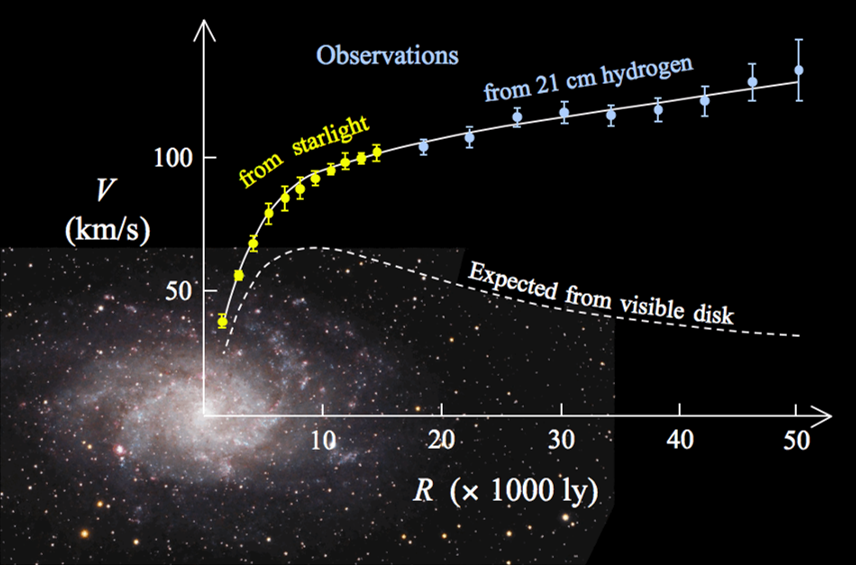
\includegraphics{figures/chapter_one/rotation_curve.png}
	\caption{Rotation curve of M33, from~\cite{Corbelli:1999af}}
	\label{fig:rotation_curve}
\end{figure}

Clearly, something is wrong with the predictions. If we assume that stars, gas, dust, and other objects visible with telescopes are all there is to a galaxy, then at large distances from the galactic center it will increasingly appear like a point mass, giving the familiar relationship $v(r) ~ r^{-1/2}$ that is Kepler's third law. In the bulge in the center of the galaxy, we see the speed increases roughly linearly with the radius, indicating a mass distribution proportional to $r^3$, or a constant density profile. However, the data clearly shows that at large $r$, the velocity is approximately constant, indicating a mass distribution proportional to $r$ or a density profile proportional to $1/r^2$. If there is something in the galaxy that would produce this distribution of mass it doesn't show up in any telescope. Additionally, the stars near the edge of the galaxy are well above the predicted escape velocity $v_{\n{esc}} = \sqrt{2}v_{\n{circ}}$, and as galaxies are stable over astronomical periods of time, they cannot be filled with objects exceding the escape velocity.

This data indicate one of two things. Either Kepler's Law and the Newtonian gravity upon which it is based are invalid on galactic distance scales, or there is some hidden mass or dark matter filling a galaxy. Supposing the first case to be true, the recourse would be to introduce modifications to gravity that only act over long distances, which has been done with some limited success~\cite{Milgrom:1983,Moffat:2005si,Worsley:2014}. In the second case, some distribution of mass must be inferred that has a negligible contribution in the inner parts of the galaxy but becomes dominant at large radii. A number of distributions have been proposed~\cite{NGW:1997,Merritt:2006} which address this rotation curve problem.

\subsection{Gravitational Lensing}

One prediction of Einstein's Theory of General Relativity is that any concentration of matter and energy will act as a lens for passing photons by distorting spacetime~\cite{}. When lensing is observed, forward modelling can be performed to estimate the distribution and amount of matter present.

\subsubsection{Strong lensing}

Provided the alignment of the stars is correctly and the foreground lensing object is sufficiently massive, the image of a distant object can be lensed strongly around the foreground object, resulting in multiple images or severe distortions. Strong lensing tends to be easy to identify (for instance, most galaxies when viewed edge-on don't bear strong resemblances to a banana). In all cases, the observed distortions require much more mass than can be observed with telescopes.

\subsubsection{Weak lensing}

In cases where the lensing object is not sufficiently dense or massive to create obvious strong lensing, weak lensing can still be observed. Weak lensing can be measured using statistical methods by creating an average shape of a galaxy in the field of view and calculating some distortion parameter. A distribution of distortion can be created, which will indicate where the greatest concentrations of mass are.

\subsection{Galaxy cluster dynamics}

The observations of the dynamics of clusters of galaxies yields fairly clear indication that dark matter must form a significant contribution to the mass of a galaxy cluster. When observations are made of clusters other than our own Local Group, a good deal of hot gas is observed. This hot gas radiates x-rays (and thus is often called hot x-ray gas), and from its luminosity both the temperature and mass can be measured. The extremely high temperatures observed are from basic energy conservation. As the gas falls into the cluster's gravitational potential well, it gains kinetic energy, which, for a gas, is equivalent to temperature. The temperature of the gas thus gives an indication of the depth of the potential well. Applying the Virial theorem (2K + U = 0) to the cluster, the kinetic energies of the component galaxies can be measured and compared to the observed potential energy. In both cases, the required potential well is much deeper than could be formed from merely the hot gas and the galaxies themselves, despite the fact that there is an order of magnitude more mass in gas than in galaxies. Indeed, the extra mass required to make the system behave is an order of magnitude greater than the mass that is observed.

\subsubsection{Bullet Cluster}

The Bullet Cluster (1E 0657-558) is an excellent example of both galaxy cluster dynamics and weak lensing, and also furnishes additional information on dark matter. Figure~\ref{fig:bullet_cluster} is a composite image of a Hubble Space Telescope (HST) image and a Chandra X-ray Observatory image. The pink is the hot x-ray gas (seen by Chandra), and forms the majority of the baryonic mass of the cluster. The powerful shock produced during the collision is clearly seen in the subcluster on the right, giving indications of the speed of the collision, and also the mass of that subcluster.

\begin{figure}[h]
	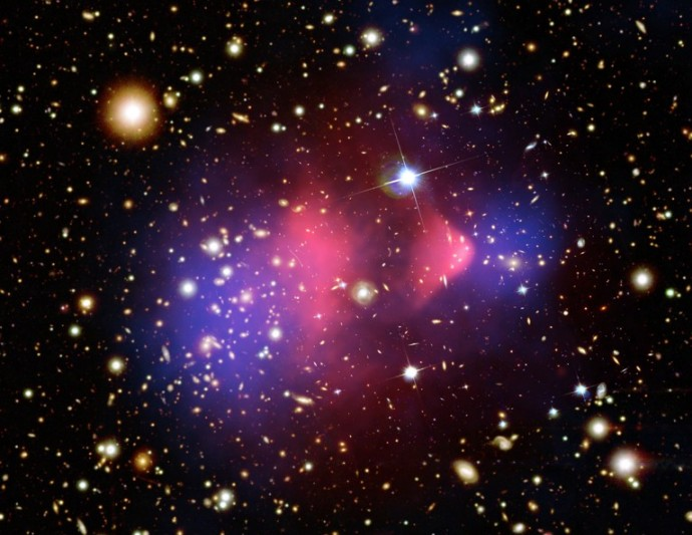
\includegraphics{figures/chapter_one/bullet_cluster.png}
	\caption{The Bullet Cluster of galaxies, from~\cite{bullet}}
	\label{fig:bullet_cluster}
\end{figure}

A good deal of information can be gleaned from a careful inspection of figure~\ref{fig:bullet_cluster}. The first thing to note is the separation of two populations of baryonic matter. In the visible wavelengths we observe the two subclusters with their galaxies largely undisturbed by their transit. The distance between galaxies in a cluster is larger than the characteristic size of a galaxy, thus a cluster is dominated by the star-less space between galaxies. When two galaxy clusters collide the chance of a direct collision between to galaxies is small, as the gaps for galaxies to slot between each other are larger than the galaxies themselves. Thus, we see that the two subclusters have been largely unaffected by their passage.

However, a respectable galaxy cluster contains far more than just galaxies. The majority of the mass comes from free hydrogen in the form of the hot x-ray gas. When two populations of gas pass through each other, they interact differently from galaxies. The gas interacts significantly as the two clouds pass through each other, which slows the gas down. Thus, as the two subclusters move away from each other post-collision, the x-ray gas will have lost some kinetic energy due to its interactions and will not leave the collision center as quickly as the stars and galaxies. This leads to a separation of the galaxies from the gas.

However, if a weak lensing study is performed on this cluster, it indicates that the lensing centers, and thus the greatest concentrations of mass, are centered around the galaxies, not the gas. This at first presents a dilemma, as the luminosities observed require that there be much more mass in gas than in galaxies. How, then, could the lensing be centered around somewhere the mass isn't? The answer is that there must be some hidden mass that accompanies each subcluster. Furthermore, we can note that this hidden mass didn't separate out with the gas, indicating that it doesn't experience significant self-interactions.

\section{Cosmological Evidence for Dark Matter}

While astrophysics tends to provide the prettier pictures, cosmology imposes more stringent numerical limits on dark matter and its distributions.

\subsection{Big Bang Nucleosynthesis (BBN)}

About a minute after the Big Bang, the universe had cooled sufficiently to allow nuclei to form and not be immediately broken apart due to the high ambient temperature. A good deal had happened in this minute, including the annihilation of all the antimatter with almost all the matter, creating the ocean of photons that is now the cosmic microwave background. It will prove convenient to define $\eta$ as the ratio between the number of baryons and the number of photons, or, as the number of photons is large, $\eta_{10} = 10^{10}\eta$. Neutrons and protons had just fallen out of numerical equilibrium due to their small difference in mass, and now existed in a ratio of about 1 neutron per 7 protons. Neutrons and protons first combined to make deuterium, then as the deuterium abundance increased, deuterium fused with deuterium to produce tritium and then with tritium to produce $^4$He. This epoch continued for just under half an hour, until expansion had driven particles far enough apart that collisions became infrequent and the temperature had decreased below the energy necessary to overcome the Coulomb repulsion between nuclei. Now, nearly all of the universe's neutrons were in helium due to its stability. Of the remaining few neutrons, most were in deuterium, with a few in $^7$Li. Due to its stability, the population of $^4$He depends very little on $\eta_{10}$, but deuterium is not strongly bound, so a smaller $\eta_{10}$ (more photons) means fewer deuterium nuclei. By measuring the primordial abundance of deuterium, this will admit a value of $\eta_{10}$ which will in turn indicate what percentage of the universe was baryons at this epoch.

\subsection{Cosmic Microwave Background (CMB)}

Pensias and Wilson were the first to turn a sensitive microwave telescope to the skies \cite{PenWil:1965a,PenWil:1965b}, and their discovery earned them the Nobel Prize in Physics in 1978. Now, the best measurements of the CMB come from satellites like WMAP and Planck. The basic data taken are nearly totally featureless and isotropic to a few parts per million as shown in Fig.~\ref{fig:cmb}a. If the average temperature of 2.7K is subtracted, a dipole term appears arising from the Sun's movement around the galaxy (Fig.~\ref{fig:cmb}b). In a sense, this indicates a favored reference frame for our universe, that is, one in which the observer is at rest relative to the CMB. If this dipole term is subtracted, the galactic contributions become clear (Fig.~\ref{fig:cmb}c). Subtracting this yields a density map of the universe when the CMB decoupled from the baryonic matter (about 380,000y after the Big Bang, Fig.~\ref{fig:cmb}d). Certain regions contain a slightly higher density than others, indicating a greater concentration of stuff. This temperature map can be expanded in the spherical harmonics and a power spectrum plotted. A cosmolical model is then fitted to this spectrum, and from this model various parameters of our universe can be extracted.

\subsection{Baryoacoustic Oscillations (BAO)}

\subsection{Structure Formation}

\section{Dark Matter in the universe today}

The burning question now is, what might dark matter be? The stuff must exist, so testable models should be proposed.

\subsection{Weakly Interacting Massive Particles (WIMPs)}

Observations (or lack thereof) of dark matter exclude interactions via electromagnetism and the strong force. However, this does not exclude weak interactions.

\subsubsection{Freezeout and the WIMP Miracle}

Supposing a population of particles existed in equilibrium with the rest of the universe at some early epoch (before BBN), as the univere expanded and cooled the production and annihilation reactions would begin to fall out of equilibrium. At some point, the universe was hot enough to allow for $\chi \bar{\chi} \leftrightarrow f \bar{f}$. However, once the temperature had dropped, the reverse reaction would become impossible, leaving $\chi \bar{\chi} \rightarrow f \bar{f}$. Eventually even this would become impossible, leaving no allowed reactions.

\subsection{Massive Compact Halo Objects (MACHOs)}

The limits on non-baryonic matter deriving from the CMB rely on the lack of detectable interaction with the CMB. However, there are more things that interact with the CMB in ways that our telescopes aren't sensitive enough to detect. The MACHO theory posits a dark matter halo filled with massive compact baryonic objects such as unowned Jupiter-sized planets, dwarfs, and small, quiet black holes. Such objects would radiate only very weakly, which would be very difficult for telescopes to directly identify. Detection of these objects is principally done through observation of micro-lensing events, where a MACHO passes in front of a background star in such a way that the gravitational lensing acts to greatly magnify the star. Modelling is then done to identify both the location and mass of the lensing object. These events have been observed but the frequency with which they happen only admits []\% of the required mass of dark matter~\cite{}.

\subsection{Axions}

Originally proposed as a solution to the strong-CP problem, axions were suggested to be dark matter candidates in [].

\subsection{Neutrinos}

The elephant in the room at this point is neutrinos. Neutrinos only interact via the weak and gravitational forces, and should be dead ringers for dark matter. Why, then, are we still looking? The answer lies in temperature. Due to the extremely low mass of neutrinos, any amount of energy greater than a few eV is sufficient to make the neutrino ultrarelativistic. Additionally, there are no mechanisms whereby a lot of neutrinos can lose a lot of energy. So, once a neutrino is created, it will tend to hold on to whatever energy it has.

Now, if the early universe was filled with ultrarelativistic matter, the structure formation we observe today could not have occurred. Any overdensity of ultrarelativistic matter will have a greater outflux than influx, which will tend to smoothe out any tendency of matter to clump under the influence of gravity. During the period of primary structure formation, most of the universe's neutrinos would have been ultrarelativistic, and so if they had been a significant component of dark matter the universe today would have a much more uniform distribution of mass, as opposed to the observed scattered delta functions. Additionally, Planck limits $\Omega_\nu$ to $<$ value~\cite{}, which is far too low to be a dominant component.

%\end{document}

% searching for DM

% chapter two: searching for dark matter

\chapter{The Search for Dark Matter}

Now that a promising model of dark matter have been proposed, some time should be spent discussing how it might be tested. There are three classes of experiments to detect WIMPs. One can try to produce them by smashing known standard model particles together. Or, one can try to observe two WIMPs smashing into each other and annihilating. Thirdly, one can try to observe a WIMP directly interacting with some standard model particle. We will discuss these three methods, their limitations, and their strengths.

\section{Production Searches}

Were one to take two standard model particles, give them together with gratuitous amounts of energy, and and smash them into one another, one generally produces a large menagerie of other particles that tend to decay fairly quickly. However, assuming there is some nonzero coupling between dark matter and the standard model, there is a probability that instead of producing other standard model particles, the collision will produce dark matter which will leave the detector without causing it to trigger. The signature of this will be missing energy and momentum from the collision. The goal, then, is to search through reams of data for these signatures. However, if there isn't a trigger there is no evidence that anything happened in the detector. This means one has to look for cases where both dark matter and standard model particles are created (so something can cause a trigger), but each additional coupling in the Feynman diagram is accompanied by a reduced probability. As the strength of these couplings is not known, this process is a little like searching for a needle in a haystack when you don't know what a needle looks like.

\section{Annihilation Searches}

Given the density of dark matter observed today, there is some finite probability that two dark matter particles will run into each other with sufficient energy to annihilate. If we happen to be fortunate enough to be pointing a telescope towards this event at the appropriate time, its signature could be detected. The goal here is to filter out which events are from known astrophysical sources and which are the dark matter signals. This is never straightforward. One could compare it to searching for a needle in a stack of slightly different needles. On numerous occasions, peaks have shown up in the data to some significance, but then vanish once a complementary experiment begins collecting data in that region of the spectrum. Additionally, the astrophysical sources are not yet completely understood.

\section{Scattering Searches}

We can continue to rotate our Feynman graph to demonstrate a scattering event. In a scattering event, the interaction between the dark matter particle and the target standard model particle will cause the target to recoil. The infomation generated in this event will be contained in the ionization of the target atom, its resulting scintillation, and the creation of phonons as the nucleus recoils into its neighboring atoms. Depending on the specifics of the detector, some combination of these can be collected. The two leading technologies in this field are based on germanium crystals and liquid noble time projection chambers (TPCs).

\subsection{Searching with Germanium}

The leading group searching for WIMPs with germanium detectors is the CDMS collaboration~\cite{}. Germanium detectors are capable of collecting the scintillation and phonons created during a WIMP scattering event.

\subsubsection{Advantages of Using Germanium}

Semiconductors have been studied for many decades and by now are very well understood. Therefore, detectors based on this technology have the advantage of a mature field of research into the systematic effects of these devices. There are a great many facilities around the world that deal with semiconducting devices. Additionally, the germanium yields excellent sensitivity to lower-mass WIMPs ($<10\1{GeV/c}^2$).

\subsubsection{Disadvantages of Using Germanium}

The most significant disadvantage of the use of germanium crystals is the practical limits to the size of crystal that can be grown. To maximize exposure, experiments generally wish for the greatest target mass possible. With germanium, this can only be accomplished by creating a large array of individual crystals. As the array will not form one large crystal structure, each component crystal and its attached detection apparati are subject to surface effects like radon or trace radioactivity in the hardware.

\subsection{Searching with Liquid Nobles}

This class of detector includes all TPCs filled with some noble elements. Xenon is the most popular element used, but argon is also used. The two main players using xenon-based TPCs are the LUX and XENON collaborations~\cite{}. The LUX detector is based in the Sanford Underground Research Facility in South Dakota, USA, while XENON is based at Laboratori Nazionali del Gran Sasso (LNGS) in central Italy. These detector types are designed to collect the scintillation and ionization created in a WIMP scattering event through the combination of a bulk liquid target and a small gas layer above it.

\subsubsection{Advantages of Liquid Nobles}

A clear advantge of the use of the TPC is the ability to scale. While calibrations for very large detectors become more challenging, it is much simpler to build a TPC with 1000kg target mass than to grow a 1000kg germanium crystal. Thus, argon- and xenon-based detectors will continue to dominate in terms of exposure. Also, the mass of xenon lends itself well to great sensitivity with higher-mass WIMPS ($>10\1{GeV/c}^2$). As this mass range is heavily favored by supersymmetric WIMP models, these detectors are poised to probe this promising region of the parameter space.

% XENON1T

% chapter three: xenon

\chapter{The XENON1T Experiment}

The leading WIMP direct detection experiment is run by the XENON collaboration, of which XENON1T is the latest version of a series of ever-larger detectors~\cite{}. Built in central Italy at Laboratori Nazionali del Gran Sasso (LNGS), XENON1T is the largest and most sensitive xenon dual-phase time projection chamber (TPC) in the world at the time of commisioning, containing 3300 kg of xenon.

\section{Operational Overview}

The operation of a dual-phase TPC is as follows. When something interacts with an atom (xenon, argon, etc) inside the detector, it will free a number of electrons, either directly or via the deexcitation of the nucleus after scattering inelastically. Some of these electrons will recombine instantly with the ion, producing scintillation light that is collected with the top and bottom PMT arrays. This signal is variably called the S1, prompt, or scintillation signal. An electric field is applied to the target volume, so some of the electrons will drift upwards towards the surface of the liquid. The ion would drift down and eventually collect electrons from the cathode mesh near the bottom of the detector, but convection currents inside the detector~\cite{Shayne's paper} dominate over the ion drift speed. Once the electrons reach the surface of the liquid, a second, much stronger electric field accelerates the electrons into the lower-density xenon gas. These energetic electrons will interact with the gas, creating more light that is again collected. This signal is variably called the S2, delayed, or ionization signal. The time difference between the S1 and S2 is the amount of time the electrons were drifing, and yields the depth or z coordinate of the interaction. The hit pattern on the top PMT array yields the (x,y) position of the event, as the PMTs directly above the S2 location will see more photons and produce a stronger signal. Figure~\ref{fig:idealized_event} shows schematically a typical event.

\begin{figure}[htb]
	\includegraphics[trim = 0 0 0 0, clip = true]{figures/chapter_three/idealized_event.pdf}
	\caption{An idealized event inside a dual-phase TPC}
	\label{fig:idealized_event}
\end{figure}

\section{System Overview}

The XENON1T detector is composed of numerous subsystems, which will be discussed here in some detail.

\subsection{Water Cherenkov Muon Veto}

The detector is housed in the center of a large tank of high-purity water, \SI{10}{m} in diameter and \SI{10}{m} in height. While the rock overburden at LNGS reduces the cosmogenic muon flux by many orders of magnitude~\cite{}, these muons typically have extremely high energies and take a long time to fully dissipate all their energy. Thus, muons can still regularly traverse the detector volume. However, by surrounding the detector with water, the muons will create Cherenkov radiation. An array of PMTs placed in the water can detect the light and a coincident event in the TPC itself tagged.

\subsection{Belt systems}

Three systems of belts are mounted in the water tank around the detector to facilitate positioning radioactive sources around the TPC to perform various tasks like electron livetime calibrations and self-shielding measurements. Two of these systems have purely vertical travel (I-belts), and the third is capable of moving a source all the way underneath the detector along a secant (U-belt).

\subsection{Gas recirculation and purification}

A large series of tubes exists to support the operation of the detector. The primary purpose of this system is to fill and empty the detector, to introduce radioactive sources into the detector for various calibrations, and to maintain the purity of the xenon in the detector by recirculating through a getter during the run.

\subsection{Electronics and DAQ}

A variety of eletronics are housed in the service building for the purpose of running the DAQ systems. An array of CAEN V1724 ADC modules digitize the signal from the PMTs and feed the output into a small server cluster that acts as the Event Builder. This software functions as the trigger and writes events to disk. These files are then transferred above ground for processing and analysis.

\subsection{TPC and Umbilical}

The TPC itself is housed inside the inner cryostat and is made of only the most radiopure materials available. The major components of the TPC are the copper field-shaping rings that help to ensure the uniformity of the drift field, the PTFE reflectors, the top and bottom PMT arrays, and the bell.

% NR calibration

% chapter four: NR calibration

\chapter{Nuclear Recoil (NR) Calibrations}

In XENON100 nuclear recoil calibrations were done through use of YBe and AmBe~\cite{}. However, the several meters of water surrounding the outer cryostat are very good at moderating and absorbing neutrons. While there's no reason why a source cannot be lowered into the water tank next to the detector or a beam pipe installed and moved into position for use~\cite{LUX}, there is a better way. YBe and AmBe both produce a spectrum of neutron energies. Also, XENON1T is big enough that it will be possible to resolve multiple scatters within the fiducial volume. This allows the possibility of using multiple scatters to perform the energy calibration. Recall elastic scattering between two objects. Given the scattering angle of the target, we can find the energy deposited using
\begin{equation}
E_{recoil} = \frac{2 E_n}{\frac{m_n}{m_{Xe}}\,(1+\frac{m_{Xe}}{m_n})^2}(1-\cos \theta)
\end{equation}

Here, $E_n$ is the energy in the incident neutron, $m_{Xe}$ and $m_n$ are the masses of the xenon and the neutron, and $\theta$ is the scattering angle. If the neutrons are monoenergetic, then a very precise nuclear recoil calibration can be performed in situ by selecting various scattering angles. Monoenergetic neutrons can easily be created from fusion reactions, of which two candidates are $^2_1D + ^2_1D \rightarrow ^3_2He (0.82 \n{MeV}) + n (2.45\n{MeV})$ (50\% branching ratio) and $^2_1D + ^3_1T \rightarrow ^4_2He (3.6\n{MeV}) + n (14.1\n{MeV})$.

A DD reaction neutron generator was acquired from NSD Fusion for the purpose of performing the nuclear recoil calibrations on XENON1T. Detectors selected to calibrate it are liquid scintillators containing the chemical EJ-301, an organic liquid polymer with high hydrogen density, manufactured by Eljen Technologies, and is identical to the older and more well-known NE-213.

\section{Pulse Shape Discrimination (PSD)}

EJ-301 is sensitive to both fast neutrons and $\gamma$ particles, but reacts differently to them. Neutron signals appear differently from $\gamma$ signals because the $\gamma$ only excites the electrons into a short-lived singlet state, where the neutron promotes the electrons into a longer-lived triplet state~\cite{}. Processing algorithms can be written to discriminate between waveforms of these two particles. The work-horse algorithm, used since the ancient times of analog processing, is known as the Charge Comparison Method~\cite{}. The advent of digital computing and cheap data storage means that data processing now does not necessarily need to be done live, allowing many other algorithms to be used for discrimination.

Traditionally, the quantification of discrimination was done by making a histogram of the discrimination parameter, fitting Guassian curves to the neutron and $\gamma$ populations, and defining a Figure of Merit as the separation of the peaks divided by the sum of the full widths at half maximum. However, the two populations in question are not generally Gaussians, so this is like trying to measure a round hole with a square peg.

\subsection{Charge Comparison Method (CCM)}

This is a method based on two integration windows or gates of the pulse. One window is called the fast or short window, the other the slow or long window. The discrimination parameter used to differentiate these two types of pulse is the ratio of the slow integral value to the fast integral value. If the end of the fast window coincides approximately with the end of the typical $\gamma$ pulse, the slow window will contain very little other than the baseline, so the discrimination parameter will be close to unity. For neutron events, however, the pulse contains a significant tail that extends beyond the end of the fast window, which is captured by the slow window. In this case, the discrimination parameter will be somewhat above unity.

\subsection{Fourier Series Analysis (DFT)}

\subsection{Laplace Transformations (LT)}

As EJ-301 exhibits decay modes with different decay constants, a Laplace transform is an effective method of identifying these modes. The Laplace transform of a function is defined as
\begin{equation} \label{eq:laplace_transform}
\mathcal{L}(s) = \int_0^\infinity \n{d}t\,f(t)e^{-st}
\end{equation}

\subsection{Fitting with Standard Events}

Once some discrimination has been done with a reasonably reliable method, it is possible to create a standard waveform of each of the neutron and $\gamma$ events. Events that pass a discrimination cut can be selected, aligned, and averaged. This will create a standard event or template waveform characterizing a detector's response to a given particle type. The advantage of this is that it will tend to reduce the effects of electronic noise. These standard events can then be fit to a captured waveform. Free parameters of the fit are a vertical offset or baseline shift, a horizontal offset or trigger shift, and a vertical scaling parameter. If the waveforms used to generate the standard events are all of a very energy band, like the $^{137}$Cs Compton edge (447 keV), the fit will serve not only to discriminate between neutron and gamma events, but will also yield an accurate measurement of the energy of the event.

\subsubsection{Generating Standard Events}

To generate these standard events, one must first identify waveforms to use. This must be done via some other method of discrimination. The standard events should be made by averaging a set of events with an extremely high purity, so aggressive cuts should be made to this end. To ensure sufficient statistics, a combination of several dozen files of data collected with the NG were used. The cuts applied to these events are a cut in energy (to select events at the $^{137}$Cs Compton edge), cuts in the CCM discrimination parameter (to select either neutron or $\gamma$ events, cuts in the cleanliness of the waveforms (RMS values of the pre- and post-pulse baselines), and a cut in the location of the peak.  The details of these cuts are given in table~\ref{tab:standard_event_cuts}.

\begin{table}
	\begin{tabular}{ l | l | l } \hline
		Cut & Events left & Acceptance \\ \hline
		None & 211528247 & 1.0 \\ \hline
		Energy & 162881 & $7.7\times10^{-4}$ \\ \hline
		Pre-pulse RMS & 162519 & \\ \hline
		Post-pulse RMS & & \\ \hline
		Neutron & & \\ \hline
		$\gamma$ & & \\ \hline
	\end{tabular}
	\label{tab:standard_event_cuts}
	\caption{Cuts used to select events to average to create standard events}
\end{table}

Next, the waveforms must all be aligned with some sample, such as the sample that triggered the event. Then, waveforms are averaged together to create a preliminary standard event. This preliminary standard event is then fit to all the waveforms that made it. Outliers to the distribution can then be identified and removed from the list of suitable events. This process can be iterated several times to improve the quality of the standard events, but the gains rapidly diminish. With sifficiently high statistics ($\mathcal{O}(10^5)$ events passing cuts), it was found that iterating resulted in negligible changes to the shape of the standard events.

\section{Neutron generator flux calibration}

The neutron generator employs inertial electrostatic confinement (IEC) to achieve fusion. In IEC fusors, a cage in the middle of the chamber is held at some high voltage. Deuterium gas is injected into the (otherwise evacuated) chamber and ionized, which causes the deuterons to fall inwards towards and then into the cage. When a sufficient population of ions has been achieved, they form a virtual anode just inside the actual cage mesh. This provides sufficient extra electric field strength to contain the deuterons and enough energy for some to achieve fusion. Half of the fusion reactions will produce the desired monoenergetic neutron, the other branching ratio is $^2_1D + ^2_1D \rightarrow ^3_1T (1.01 \n{MeV}) + p^+ (3.02 \n{MeV})$. The reaction rate depends on the high voltage and current applied to the confining cage, so to understand the operation of the neutron generator, the response to these parameters must be understood.


% ER calibration
% chapter 5: ER calibrations

\chapter{Electronic Recoil (ER) Calibrations}

Liquid xenon is particularly good at absorbing $\beta$ and $\gamma$ radiation, so the methods used in XENON100 of placing sources on the exterior of the detector simply are no longer feasible for XENON1T due to the \SI{7}{cm} of xenon between the TPC and inner cryostat. The solution, then, is to introduce some radioactive source into the detector itself and perform calibrations from the inside.

However, one must very carefully select the isotopes used. Obviously, the decay chain must contain some radiation useful for calibration. The isotope selected must injectable into the detector in some manner, but more importantly, the activity must be removeable as well. Removing stuff from the detector can either be accomplished by recirculation or by letting the isotope decay.

An excellent candidate for the internal ER calibrations is $^{212}$Pb. This isotope occurs in the decay chain of $^{220}$Rn, which is also a noble element and therefore can easily be mixed into the xenon. $^{212}$Pb decays to the ground state of $^{212}$Bi with a branching ratio of 11.9\% and a Q-value of \SI{570}{keV}, which means a reasonable percentage of $\beta$ particles will have the required low energies. Finally, there is nothing long-lived in the rest of the decay sequence (as shown in Table~\ref{tab:th_chain}), which ends with $^{208}$Pb.

\begin{table}[ht]
	\renewcommand{\arraystretch}{1.2}
	\begin{tabular}{| c | c | c | c | c |}
		\hline
		Isotope & Half-life & Decay mode & Q-value (keV) \\ \hline
		$^{232}$Th & $1.41\times10^{10}$ yr & $\alpha$ & 4081 \\ \hline
		$^{228}$Ra & 5.7 yr & $\beta$ & 46 \\ \hline
		$^{228}$Ac & 6.15 hr & $\beta$ & 2124 \\ \hline
		\Th & 1.9 yr & $\alpha$ & 5520 \\ \hline
		\Ra & 3.66 d & $\alpha$ & 5989 \\ \hline
		\Rn & 55.6 s & $\alpha$ & 6405 \\ \hline
		$^{216}$Po & 0.145 s & $\alpha$ & 6906 \\ \hline
		\Pb & 10.6 h & $\beta$ & 570  \\ \hline
		\multirow{2}{*}{$^{212}$Bi} & \multirow{2}{*}{61 m} & $\alpha$ (36\%)& 6207 \\
		& & $\beta$ (64\%)& 2252 \\ \hline
		$^{212}$Po & 299 ns & $\alpha$ & 8954 \\ \hline
		$^{208}$Tl & 3.1 m & $\beta$ & 4999 \\ \hline
		$^{208}$Pb & \multicolumn{3}{|c|}{Stable} \\
		\hline
	\end{tabular}
	\caption{The decay chain of primordial thorium, sometimes called the 4n series}
	\label{tab:th_chain}
\end{table}

\section{Introduction}\label{sec:introduction}

Various low-background experiments are searching for rare events such as neutrinoless double-beta decay~\cite{Pandola:2014naa} or dark matter scatters~\cite{Undagoitia:2015gya}. Time projection chambers (TPCs) using liquid noble elements such as argon and xenon are at the forefront of these investigations~\cite{Albert:2015ekt,Aprile:2013doa,Akerib:2015rjg,Amaudruz:2014nsa,Calvo:2015uln,Agnes:2015ftt}. As these detectors become large, new challenges arise in accurately calibrating their response throughout the detection volume. For example, the XENON1T detector~\cite{Aprile:2015uzo} is a TPC $1\1{m}$ in diameter and in height, much larger than e.g. the $70\1{mm}$ mean free path of the $1.3\1{MeV}$ $\gamma$ from $^{60}$Co. Thus, calibration of the entire fiducial volume with external sources is no longer feasible.

One solution is to directly mix a radioactive isotope into the liquid noble element. In liquid xenon, $^{83m}$Kr has been proposed~\cite{Hannen:2011,Manalaysay:2009yq,Kastens:2010} and used~\cite{Akerib:2013tjd} to achieve a low-energy $\gamma$-line calibration throughout the detector. Tritiated methane has been used as a low-energy beta source~\cite{Akerib:2013tjd}. While this source has the advantage that all decays are in the low-energy range interesting to a dark matter search, it suffers from the disadvantage that the activity does not decay by itself but must be extracted from the liquid target by a hot zirconium getter in a xenon recirculation loop~\cite{Akerib:2015wdi}. This introduces an additional time constant that will get longer as the size of these detectors increases.

Here, we study a source containing \Th~that emanates \Rn~($T_{1/2}=56\1{seconds}$), which in turn can be mixed into the liquid target. The \Rn~decay chain is versatile, producing $\alpha$-, $\beta$-, and $\gamma$-radiation that makes this source interesting for a wide range of applications: The source is the ideal calibration source for intrinsic $^{222}$Rn backgrounds that are notoriously difficult to control in low-background experiments. (2) High-energy alphas~\cite{WeberM:2013,Albert:2015vma} and $^{212}$Bi/$^{212}$Po decays~\cite{Bellini:2012qg} can be used to accurately understand intrinsic backgrounds. The relatively short half-life of $^{216}$Po (145~ms) allows for the measurement of currents or liquid flows within the bulk of the detector volume. Using position reconstruction algorithms that yield the positions of the decays of \Rn~and $^{216}$Po together with the time difference between these two decays, allows for a measurement of the drift velocity of polonium ions~\cite{Albert:2015vma}. Thus, currents within the bulk of the detector can be mapped to identify possible dead regions that do not participate in the recirculation of the active volume through purification systems. Additionally, the high-energy $\alpha$ lines can be used to probe regions in a detector with poor light or charge collection efficiency. Further, the $^{208}$Tl decay produces a $2.6\1{MeV}$ $\gamma$-line that can be used to calibrate the Q-value of the $^{136}$Xe neutrinoless double-beta decay~\cite{Auger:2012}. Finally, $\beta$-decays of the chain that go to the ground state can be used to calibrate the low-energy response of dark matter detectors. While the high Q-value of the $^{212}$Bi $\beta$-decay (2.2~MeV) and short life-time of the daughter $^{212}$Po (300~ns) render that decay unsuitable for this purpose, the $\beta$-decay of \Pb~(12.3\% branching ratio to ground state, Q-value 570~keV) is very suitable for this task, as shown in Figure~\ref{fig:pb212spectrum}.

\begin{figure}[htb]
\centering
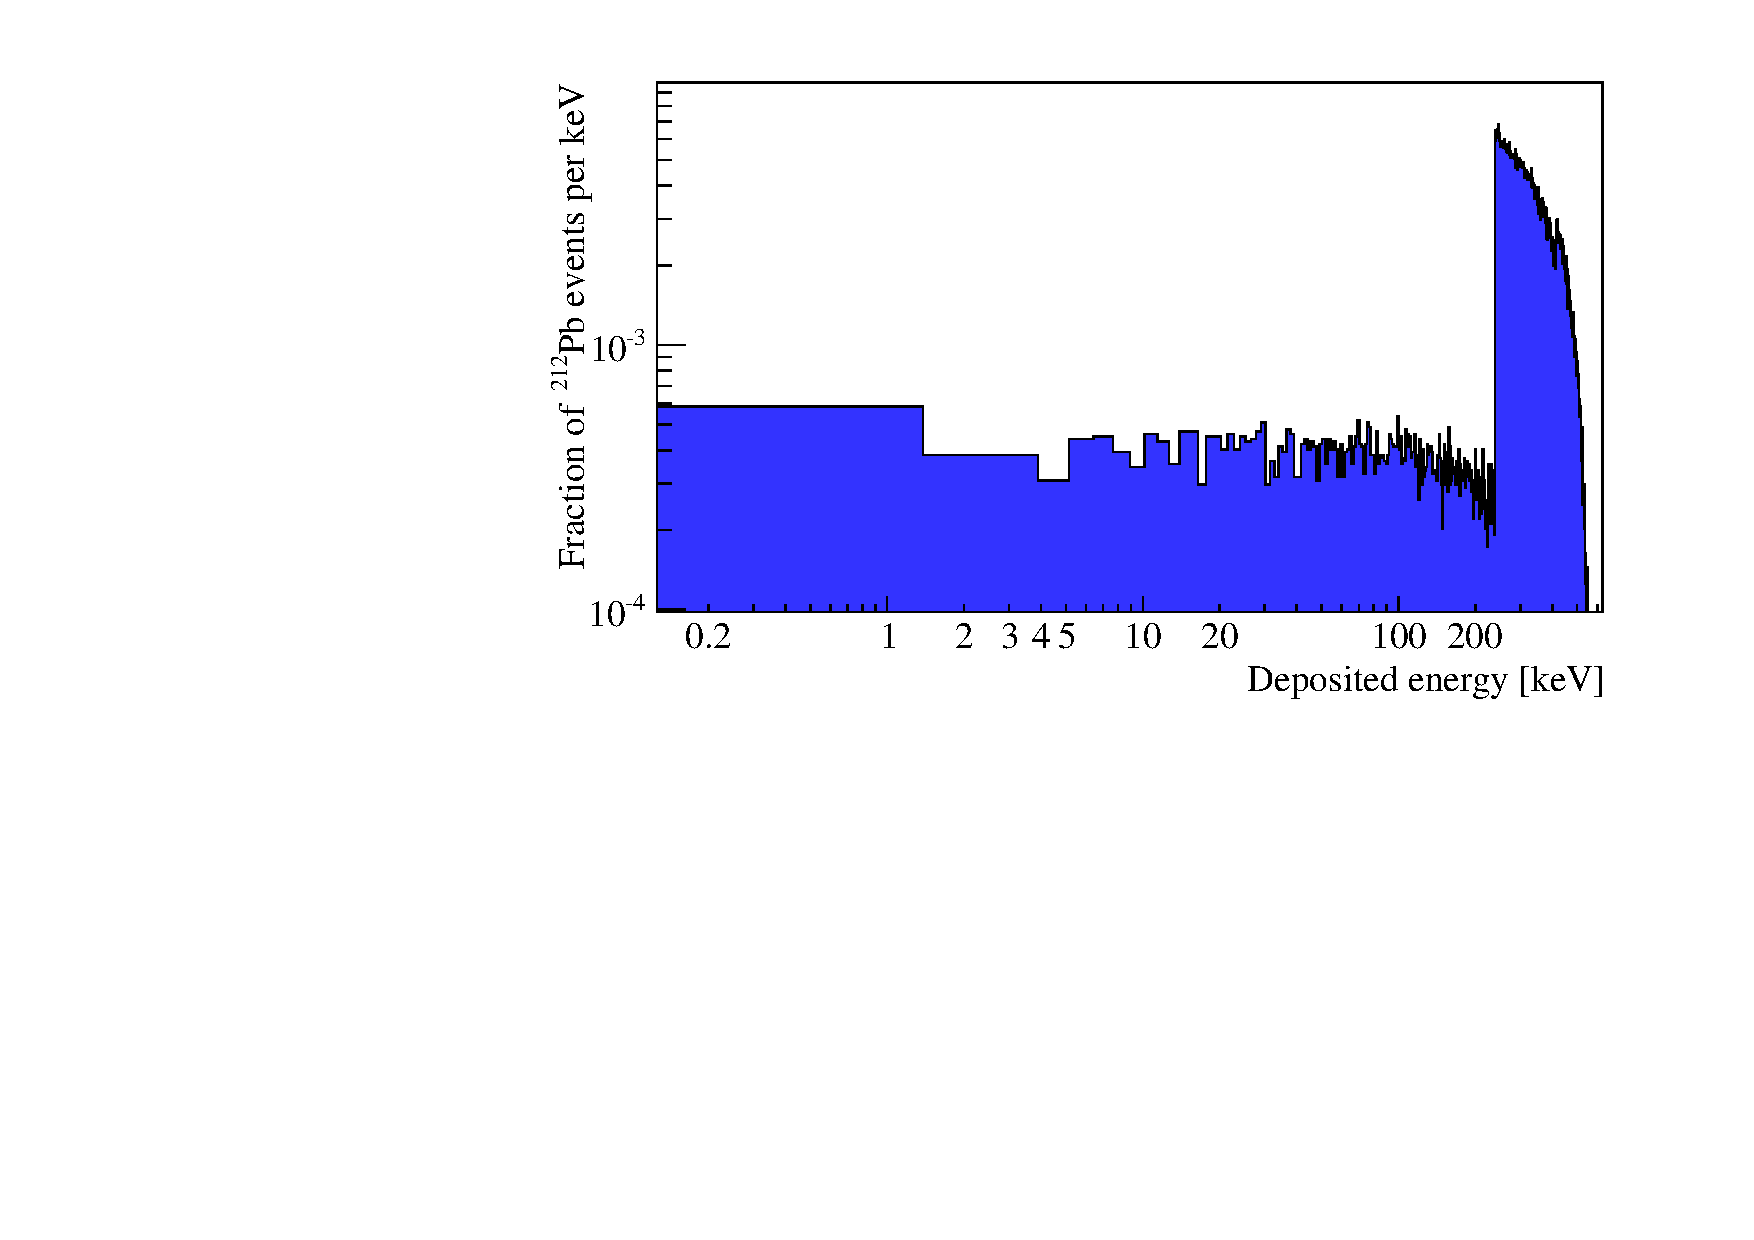
\includegraphics[trim = 5 0 50 15, clip = true,width = 0.8\columnwidth]{figures/chapter_five/pb212_spectrum.pdf}
\caption{A simulation of the $\beta$-spectrum of \Pb. The feature at 240 keV is due to decay modes with an associated $\gamma$ that adds to the energy observed in the decay.}
\label{fig:pb212spectrum}
\end{figure}

A major advantage of our source is that the time scale of the \Rn~decay chain is dominated by the relatively short half-life of \Pb~($T_{1/2}=10.66\1{hours}$). Thus, the introduced activity can completely decay away within a few days, making this source useful even for the largest anticipated liquid detectors~\cite{Baudis:2012,Akerib:2015cja,Franco:2015pha}. As both \Th~($T_{1/2}=1.9\1{years}$) and \Ra~($T_{1/2}=3.6\1{days}$) have much longer half-lives, emanation of these isotopes from the source must be limited. Also, isotopic contaminations with $^{230}$Th in the $^{228}$Th source itself can lead to the emanation of $^{222}$Rn ($T_{1/2}=3.8\1{days}$) which has to be avoided.

Here, we use a variety of methods to derive limits on the release of long-lived isotopes, and demonstrate that these sources are suitable for the calibration of even next-generation low-background experiments. Open \Rn~sources were produced by electroplating thorium nitrate, $\n{Th}(\n{NO}_3)_4$, onto the center of a $30\1{mm}$ diameter stainless steel disk in a bath of 1M nitric acid ($\n{HNO}_3$). A ring of width 2.5~mm around the edge of the disk was left for mounting purposes. The activity was $40\1{kBq}$ as of March, 2015. Each source is held in a small stainless steel vessel to attach it to a noble gas recirculation system using 1/2"~VCR piping, see figure~\ref{fig:th228source}.

\begin{figure}[htb]
\centering
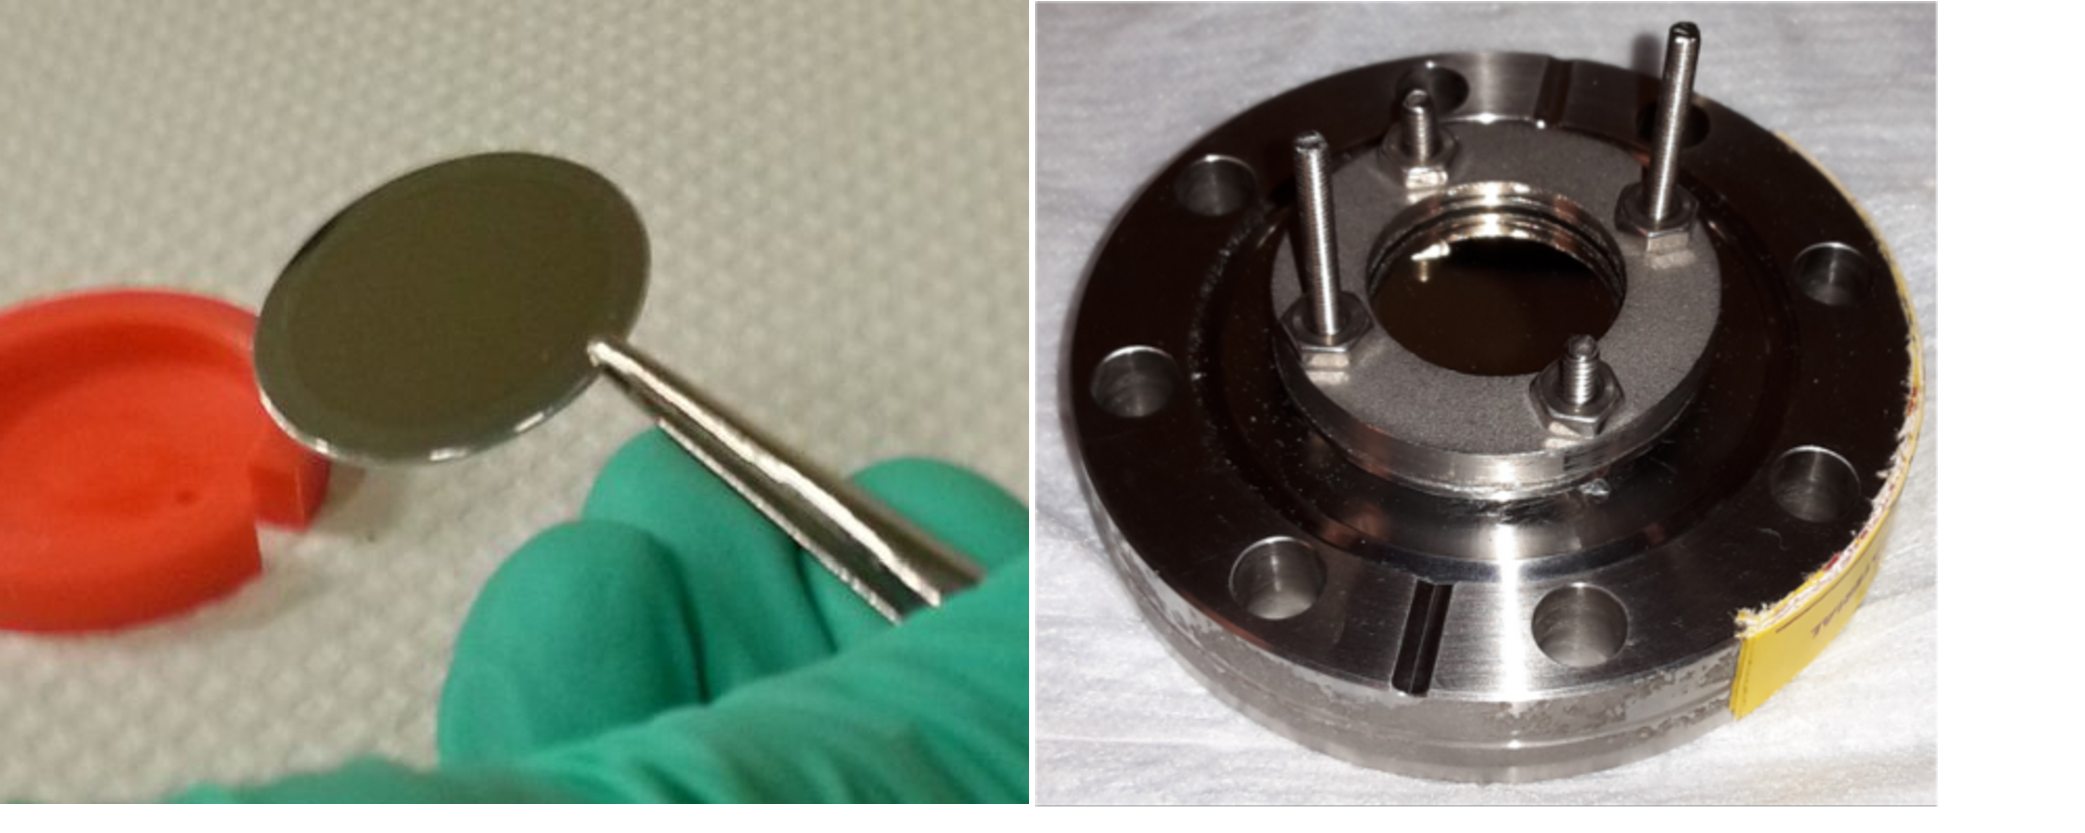
\includegraphics[trim = 5 10 65 0, clip = true,width = 0.8\columnwidth]{figures/chapter_five/source_image.pdf}
\caption{\Th~is deposited onto a $30\1{mm}$ stainless steel disc (left). It is held in a simple emanation vessel (right) for mounting on a noble gas system.}
\label{fig:th228source}
\end{figure}

\section{$\gamma$-Measurements of Filter Deposition}
\label{sec:tuv}

% TUV measurement
The source was tested for the release of \Ra~and \Th~using a standard procedure. Nitrogen was flushed through the source vessel for 96 hours. A filter of type ML050/0 was mounted inline $18\1{cm}$ after the source, containing a filter paper on which any released radionuclides could be deposited. This filter paper was then tested for $\gamma$-activity with a high-purity germanium detector. A first measurement was made immediately after exposure, and a second measurement a week later, see Table~\ref{tab:tuv}.

\begin{table}[htb]
\centering
\caption{Measurements of radionuclide release from the \Rn~source collected in filter paper.}
\label{tab:tuv}
\renewcommand{\arraystretch}{1.2}
\begin{tabular}[c]{llcc}
\hline\hline
\multicolumn{2}{l}{Measurement} & 1 & 2 \\
\multicolumn{2}{l}{Time after exposure} & Immediate & 1 week \\
\multicolumn{2}{l}{Livetime} & $375\1{s}$ & $11\,500\1{s}$ \\ \hline
\multirow{5}{*}{Activity/Bq}
& \Th & $<35$ & $<1.97$ \\
& \Ra & $<6$ & $<0.61$ \\
& \Pb & $87\pm11$ & $<0.07$ \\
& $^{212}$Bi & $84\pm34$ & $<0.68$ \\
& $^{208}$Tl & $28\pm5$ & $<0.07$ \\
\hline\hline
\end{tabular}
\end{table}

Both the exposure time and the time between measurements are significant compared to the half-life of \Ra. We account for both the decay during these intervals as well as the production of \Ra~from the decay of \Th. The week between the two measurements is more than 15 half-lives of \Pb, hence any recorded activity of its daughters $^{212}$Bi or $^{208}$Tl in the second measurement would have been from the decay of \Ra, not any initial population of \Pb. We use the lowest measurement (here, \Pb) to constrain the release of \Ra~from the source to $<0.43\1{atoms/s}$ and that of \Th~to or $<22\1{atoms/s}$. Scaling these values for the activity of the source yields a stray emanation of $<0.66\1{atoms/min/kBq}$ \Ra~and $<34\1{atoms/min/kBq}$ \Th. We choose these units (atoms/min/kBq) to account for the decay of the sources over the time the various measurements were made, and to allow comparisons between the sources.

The obvious limitation of this measurement is that there may have been radium or thorium released by the source but not caught by the filter, in which case the given limits must be scaled by the efficiency of the filter. Additionally, any thorium or radium plated out on the pipes connecting the source vessel and the filter would not show up in this measurement.

% Jochen's measurements
A similar but more sensitive experiment was performed by pumping nitrogen at 1 standard liter per minute (slpm) for 9 days in a closed loop through the \Rn~source vessel. The source was followed by a MILLEX-FG 50 filter at a distance of \SI{8}{cm}, containing a $0.2\1{\mu m}$ PTFE filter membrane. The exposure time brought any released \Ra~nearly into equilibrium on the filter and gave potential \Th~more time to deposit itself. After exposure, the filter membrane was tested for $\gamma$-activity with high-purity germanium detectors~\cite{Budjas:1,Budjas:2}. A spectrum of these measurements is shown in figure~\ref{fig:gammaspectrum}. A simulation of the germanium crystal detector geometry performed in GEANT4~\cite{Geant4} indicated an efficiency of 6.5\% at \SI{240}{keV}.

\begin{figure}[htb]
\centering
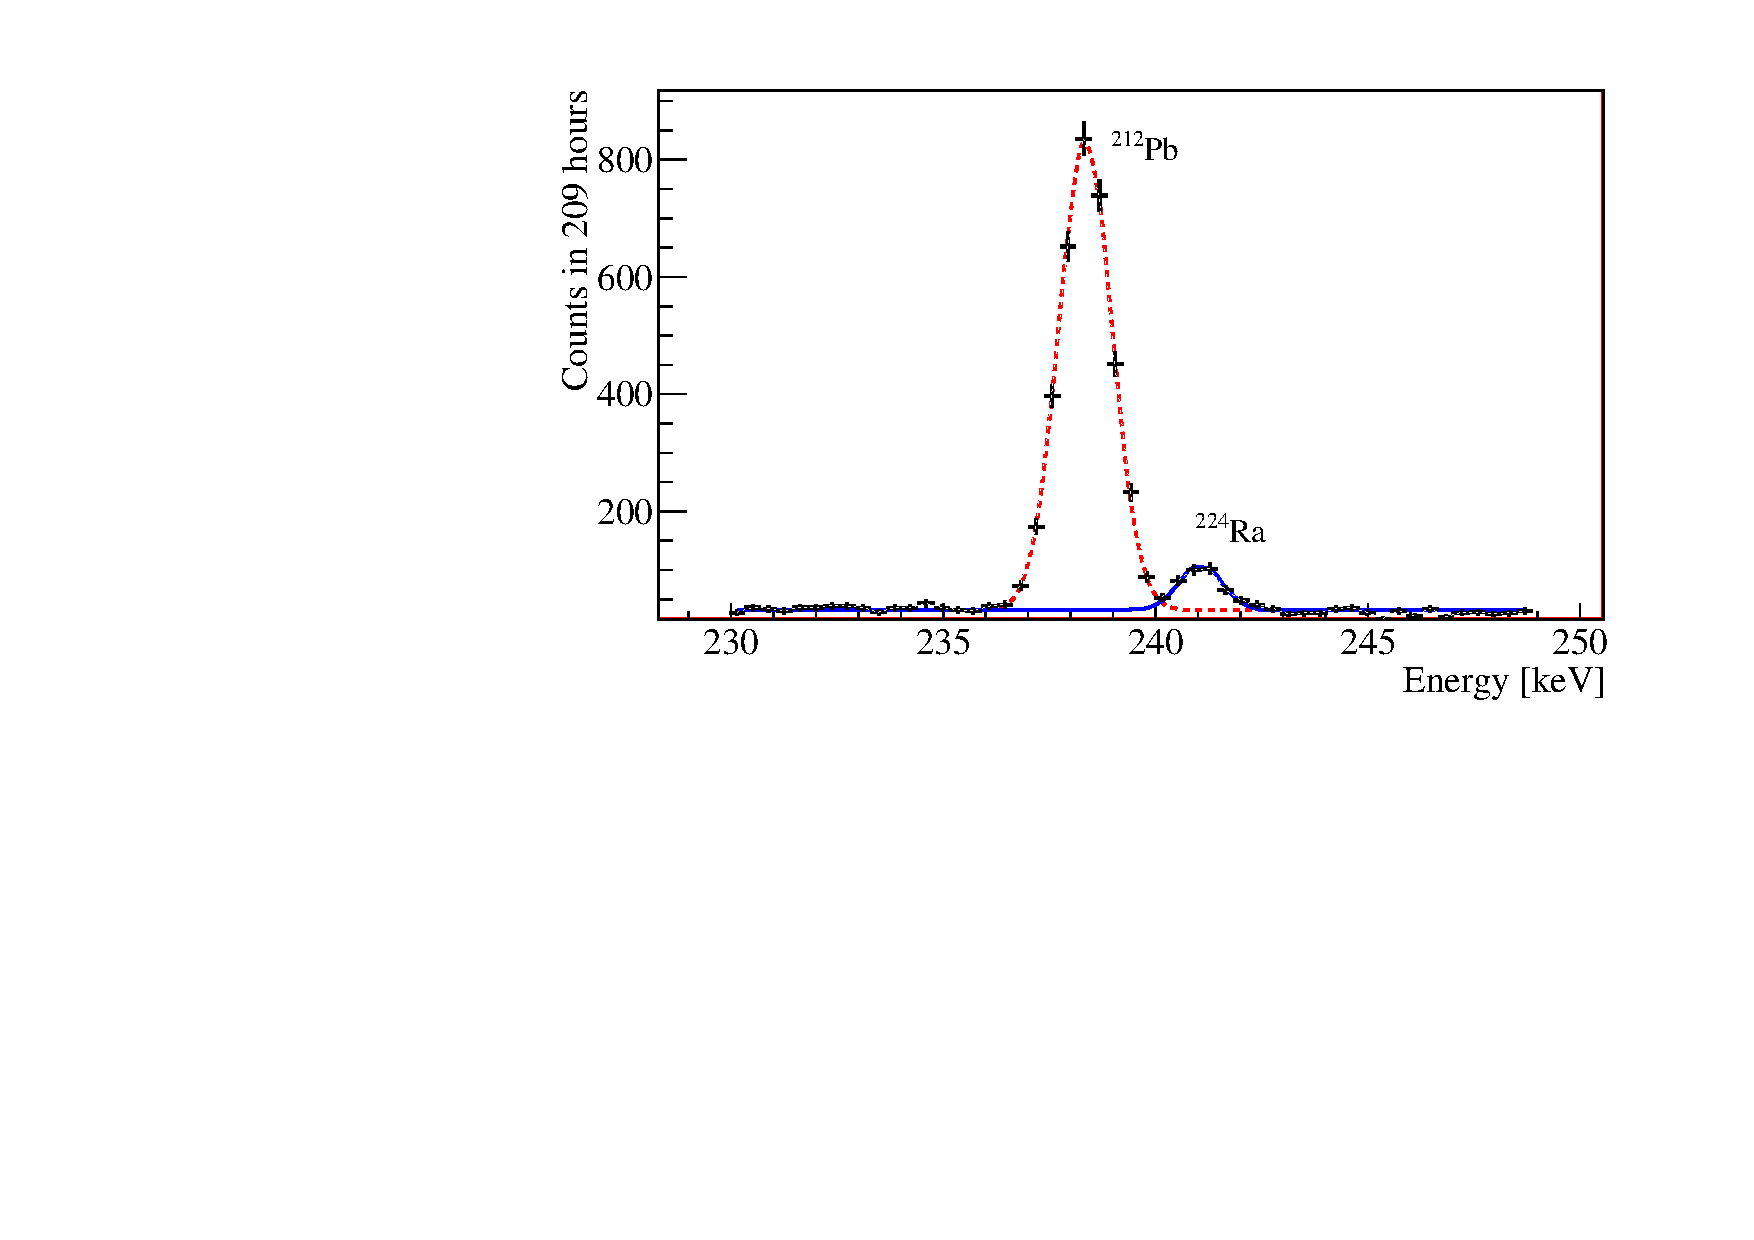
\includegraphics[trim = 15 0 50 20, clip = true,width = 0.8\columnwidth]{figures/chapter_five/ge_spectrum.pdf}
\caption{Gamma spectrum taken of the filter 7.2 days after exposure showing the \Pb~line at \SI{238.6}{keV} and the \Ra~line at \SI{241.0}{keV}. The dashed and solid lines are from a fit to the data.}
\label{fig:gammaspectrum}
\end{figure}

A week after exposure most of the \Pb~has decayed and measurements become sensitive to \Ra. A measurement with a livetime of 208 hours yielded a \Ra~activity of $(1.0\pm0.3)\1{Bq}$ on the filter at the end of exposure. A second measurement was done forty-two days after exposure, at which point the \Ra~deposited on the filter should have decayed to $3\times10^{-4}$ of the initial population. Thus, any measured \Ra~activity could be attributed to residual \Th. We calculate upper limits (90\% CL) of 2.5 mBq for \Th~and 2.4 mBq for \Ra~on the filter. These activities convert to emanation rates of $(1.9\pm0.6)\1{atoms/min/kBq}$ \Ra~and $<0.4\1{atoms/min/kBq}$ \Th.

\section{$^{222}$Rn Emanation Measurement}

Potential traces of $^{226}$Ra or $^{230}$Th in the \Rn~source would lead to a non-negligible emanation of the long-lived radon isotope $^{222}$Rn, which must be avoided. We applied ultra-low background proportional counters as described in~\cite{zuzel_llrmt} to measure directly the $^{222}$Rn emanation rate of the source. For this purpose the source was connected to a 1 liter stainless steel buffer volume, separated by a valve. The setup was evacuated and the valve was opened such that \Rn~and $^{222}$Rn from the source could emanate into the buffer volume. After some days the valve was closed and the buffer volume was separated from the source. When all \Rn~had decayed, the $^{222}$Rn was extracted from the buffer volume and filled to a proportional counter in which the alpha decays of $^{222}$Rn and its daughters were counted.

We repeated the measurement three times with a small modification in the the third measurement: Instead of emanating into vacuum, we filled 1.5 bar of helium in the buffer volume to check whether there is a difference between radon emanation into gas and into vacuum. It turned out that this is not the case as all three measurements are in good agreement and compatible with zero. The combined result is a $^{222}$Rn emanation rate from the \Rn~source of $<55\1{\mu Bq}$.

\section{Si PIN Diode Measurements}
\label{sec:diode}
% radon monitor
A direct measurement of the \Rn~source was performed with a custom-developed radon monitor. It consists of a 3-liter vacuum-tight stainless steel vessel containing a \SI{2}{cm} square windowless Si PIN diode from Hamamatsu. A high voltage of \SI{1.5}{kV} collects the charged ions resulting from the decays of \Rn~onto the surface of the diode, where the $^{216}$Po decay can be detected with an efficiency of about 35\%. The radon detector was calibrated using a $^{226}$Ra solution with a known activity of $(25\pm1)\1{Bq}$ by bubbling nitrogen through the solution, thus obtaining a known activity of $^{222}$Rn.

The \Rn~source was placed directly inside the radon monitor, which was filled with air, and \Rn~was allowed to reach equilibrium. Assuming the same collection efficiency of $^{222}$Rn and \Rn, an emanation of $(1750\pm50)\1{Bq}$ \Rn~was determined. After 10~days, the \Rn~source was removed from the radon monitor and the vessel evacuated, and all collected ions on the surface of the Si PIN diode were left to decay. Six days after the removal of the source, all \Rn~activity would be due to emanated \Ra~collected on the surface of the diode. The emanated \Ra~activity was calculated to be $(2.1\pm0.7)\1{Bq}$ and the \Th~activity as $<50\,\mu\n{Bq}$ at the point when the source was removed, which corresponds to a \Ra~emanation rate of $(3.9\pm1.3)\1{atoms/min/kBq}$ and a \Th~rate of $<0.008\1{atoms/min/kBq}$.

% absolute emanation
To further determine levels of emanation, the source was placed directly facing a Hamamatsu windowless Si PIN diode that acts as an alpha spectrometer~\cite{Bray}. The source and diode were placed in a small vessel separated by only $8\1{mm}$. The vessel was then evacuated, and the source was left for five days to deposit material onto the surface of the diode. The source was then removed and the atoms deposited onto the diode were left to decay under vacuum. Figure~\ref{fig:pindiodespectrum} shows the total activity in the diode above $1\1{MeV}$ decaying away after the removal of the source.

\begin{figure}[htb]
\centering
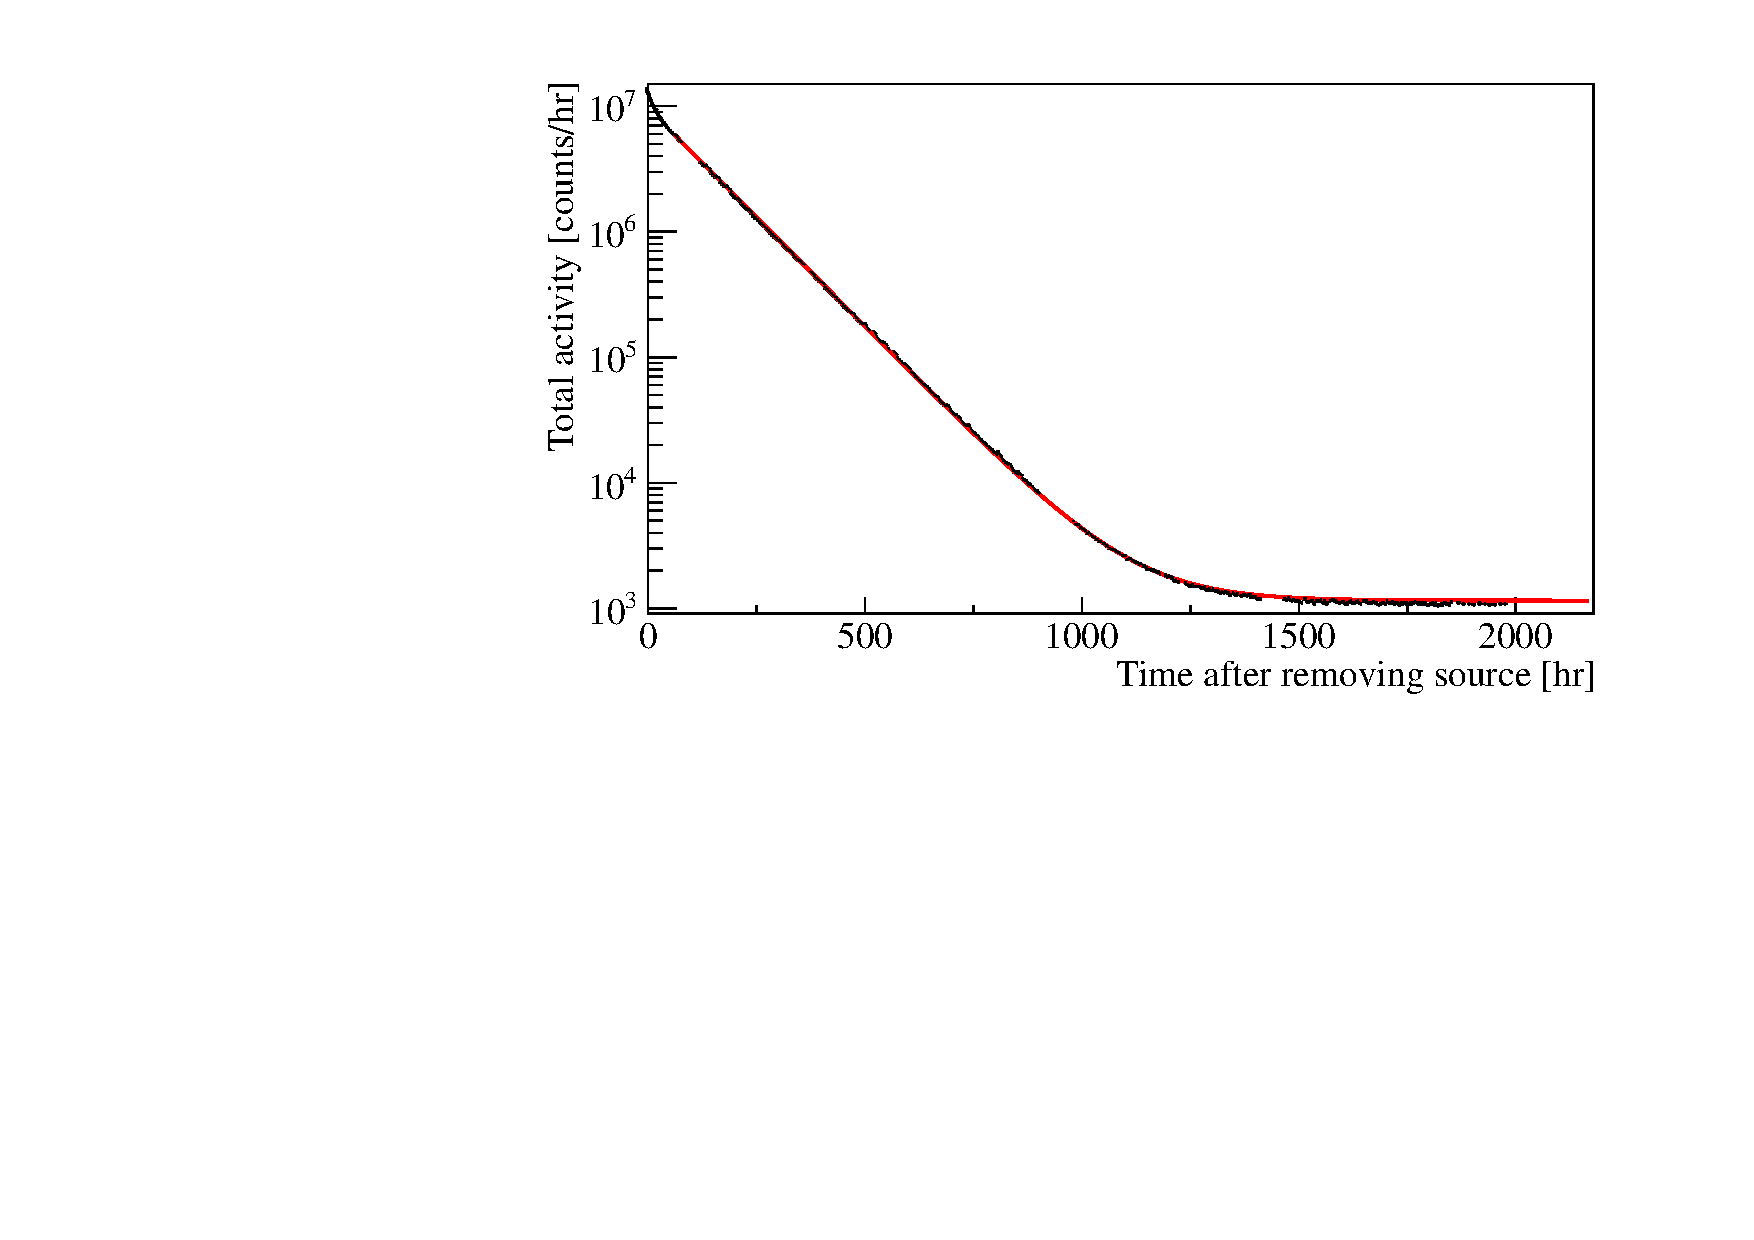
\includegraphics[trim = 5 5 55 20, clip = true,width = 0.8\columnwidth]{figures/chapter_five/opensourceactivity.pdf}
\caption{Total activity in the Si PIN diode above 1 MeV. The data points include statistical error bars, barely visible on this scale. The line is the fit of an exponential plus constant baseline.}
\label{fig:pindiodespectrum}
\end{figure}

An exponential decay plus a constant baseline is fit to this data, yielding a decay constant in agreement with the accepted half-life of \Ra, and a residual background of $(1128\pm3)\1{hr^{-1}}$. Extrapolating the curve backwards and scaling for the fraction of total activity that is \Ra, we can calculate the emanation rate of \Ra~onto the surface of the diode to be $(924.0\pm0.3)\1{s^{-1}}$. Two months after removing the source, the initial population of \Ra~will have decayed away, so the background value inferred from the fit is due to a combination of intrinsic backgrounds (here, measured to be negligible) and released \Th. By measuring the activity in the relevant portion of the spectrum, we find a \Th~activity of $(0.097\pm0.003)\1{Bq}$, or $(8.4\pm0.3)\times10^6\1{atoms}$. Given the exposure time, this corresponds to a \Th~emanation rate of $(18.3\pm0.6)\1{s^{-1}}$ onto the surface of the diode. Simulation with GEANT4 yields a geometric efficiency for deposition of 0.13, which allows us to scale the emanation rates of the source to $(4.5\pm0.2)\1{atoms/s/kBq}$ \Th~and $(282.1\pm0.1)\1{atoms/s/kBq}$ \Ra.

% Argon flushing measurement
\section{$\gamma$-Spectroscopy of Pipe Contamination}
\label{sec:flush}

A test of radium plate-out was performed by flushing argon from a high-pressure tank through a pressure regulator, the source vessel, and then a copper pipe of $6\1{mm}$ diameter and $50\1{cm}$ length. The argon flow averaged $6\1{slpm}$ though with sizeable fluctuations. After 41~hours of flushing, the copper pipe was cold-welded shut at both ends to seal in any materials deposited on the inner surface, and swiftly transported for measurement using our low-background germanium counters. Several measurements were done over the course of about two months to determine the $\gamma$-activity of the copper pipe. The results of the measurements are given in Table~\ref{tab:flush_meas}.

\begin{table}[htb]
\centering
\caption{Results of the measured $\gamma$-activity in the cold-welded copper pipe after flushing argon through source and pipe.}
\label{tab:flush_meas}
\renewcommand{\arraystretch}{1.2}
\begin{tabular}{llccc}
\hline\hline
\multicolumn{2}{l}{Measurement} & 1 & 2 & 3 \\
\multicolumn{2}{l}{Time after exposure} & 10 hours & 7 days & 68 days \\
\multicolumn{2}{l}{Livetime} & $76\,733\1{s}$ & $897\,820\1{s}$ & $357\,802\1{s}$ \\ \hline
\multirow{2}{*}{Activity [Bq]}
& \Ra & N/A & $0.25\pm0.03$ & $<0.088$ \\
& \Pb & $13.8\pm0.1$ & $0.215\pm0.005$ & $<0.088$ \\
\hline\hline
\end{tabular}
\end{table}

The interpretation of these data is done in a very similar way to that presented in the previous section. The first measurement started approximately 1 half-life of \Pb~after exposure, so any amount deposited on the pipe would still be observable. By the time the second measurement was started, a week had passed ($>$15 half-lives), so any initial \Pb~would have decayed to a negligible amount, making the measurement sensitive to potential \Pb~from the decay of \Ra. The interval between exposure and the third measurement is many half-lives of \Ra, making the measurement sensitive to potential contamination from the parent \Th~in the copper pipe.

\begin{table}[htb]
\centering
\caption{Calculated values and limits on \Ra~and \Th~release from deposition in the copper pipe after argon flushing.}
\label{tab:flush_limits}
\renewcommand{\arraystretch}{1.2}
\begin{tabular}{lcc}
\hline\hline
Isotope & Activity after exposure & Emanation rate \\ \hline
\Pb & $(26.0\pm0.2)\1{Bq}$ & N/A \\
\Ra & $(0.95\pm0.11)\1{Bq}$ & $(1.53\pm0.04)\1{atoms/min/kBq}$ \\
\Th & $<0.093\1{Bq}$ & $<47\1{atoms/min/kBq}$ \\
\hline\hline
\end{tabular}
\end{table}

Indeed trace amounts of \Ra~appear to have come off the source in this experiment. While the overall activity is very small, it motivates the use of an additional filter just after the source vessel for the calibration of low background detectors.

% Alpha spec at Purdue
\section{Measurements of Filter Efficacy}
\label{sec:filter}

In order to assess the performance of various filters in limiting the release of \Ra~from the \Rn~source, the source vessel was connected to a xenon gas system. Xenon gas was recirculated through various configurations involving the \Rn~source vessel, filters, and a Si PIN diode as an $\alpha$-spectrometer~\cite{Bray}. The source was exposed to the xenon gas stream for a few days, then bypassed, and the decaying activity monitored to measure any released radium. Two filter types were tested for their ability to remove radium from the gas stream. The first filter was a Swagelok F-series 0.5-micron sintered filter, the second was a Swagelok SCF-series ceramic filter.

The source vessel was connected directly to the sintered filter and then to the Si PIN diode with about $1\1{m}$ of 1/4" stainless steel pipe. For the ceramic filter, the extra piping was reduced to 8 cm. Xenon gas at $1\1{barg}$ was recirculated through the gas system at $5\1{slpm}$ for the sintered filter and $10\1{slpm}$ for the ceramic filter. After exposure with the sintered filter in line, the source and filter were bypassed and recirculation continued through the detector vessel for several weeks. After exposure with the ceramic filter, recirculation was stopped and the activity deposited in the detector vessel left to decay. Figure~\ref{fig:bipo} shows the activity of coincident $^{212}$Bi-$^{212}$Po (BiPo) activity in the Si PIN diode for the measurement of the ceramic filter from when the source was opened to three days after the source was closed, when the detector vessel was evacuated.

\begin{figure}[htb]
\centering
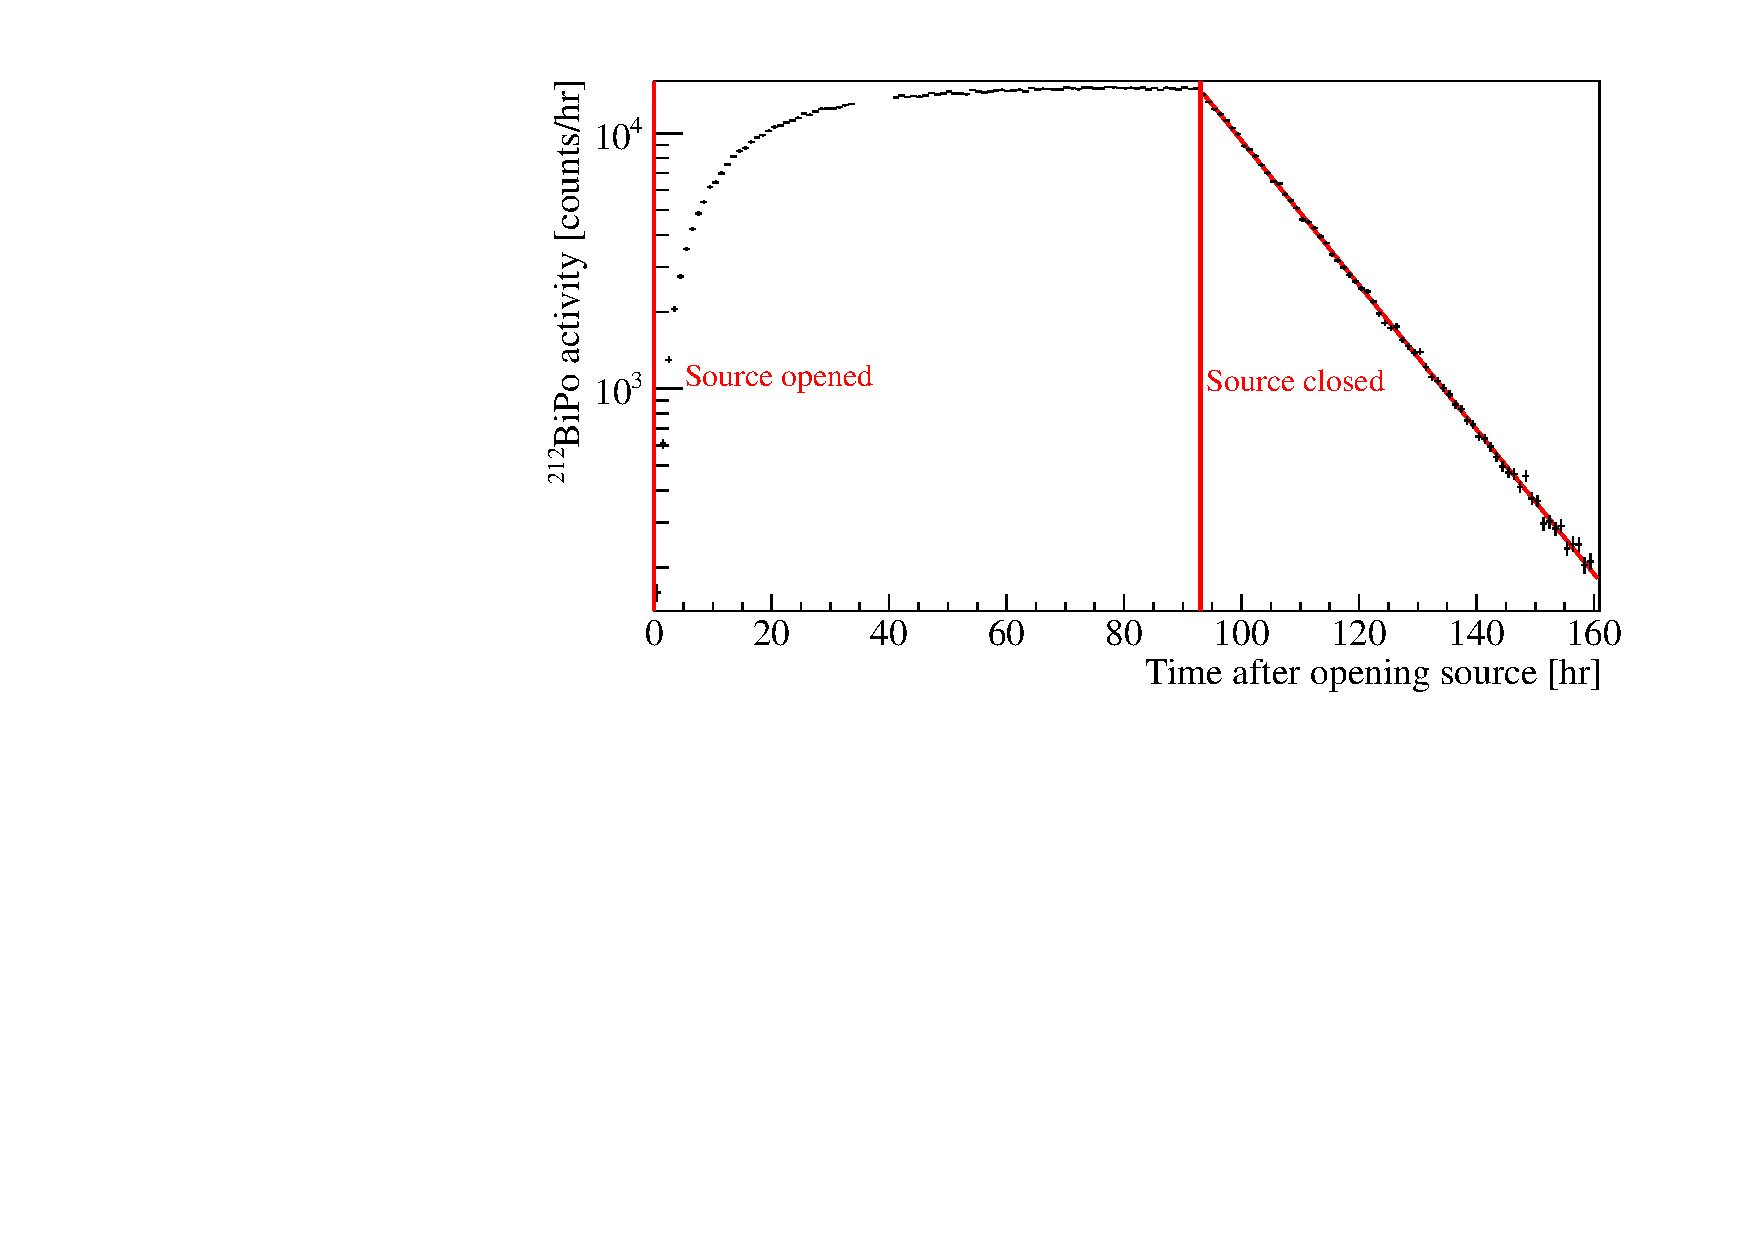
\includegraphics[trim = 5 5 40 15, clip = true,width = 0.8\columnwidth]{figures/chapter_five/bipo_activity.pdf}
\caption{Activity of $^{212}$BiPo in the Si PIN diode during and after flushing xenon through the ceramic filter. An exponential was fitted to the decaying part, yielding a half-life of $(10.64\pm0.05)\1{h}$ in excellent agreement with the \Pb~half-life of $(10.64\pm0.01)\1{h}$~\cite{Firestone}.}
\label{fig:bipo}
\end{figure}

The activity in the Si PIN diode was monitored as the released \Pb~decayed to background levels. A summary of the results are given in Table~\ref{tab:filter_limits}. About 14 half-lifes after closing the source the \Pb~has almost completely decayed to background levels, at which point any measurement would be sensitive to the release of \Ra. The background rate of $^{212}$BiPo events was found prior to these measurements to be $(42\pm7)\1{\mu Bq}$. Figure~\ref{fig:bipo_background} shows the decay for the measurement of the sintered filter, along with a fitted exponential and constant.

\begin{figure}[htb]
\centering
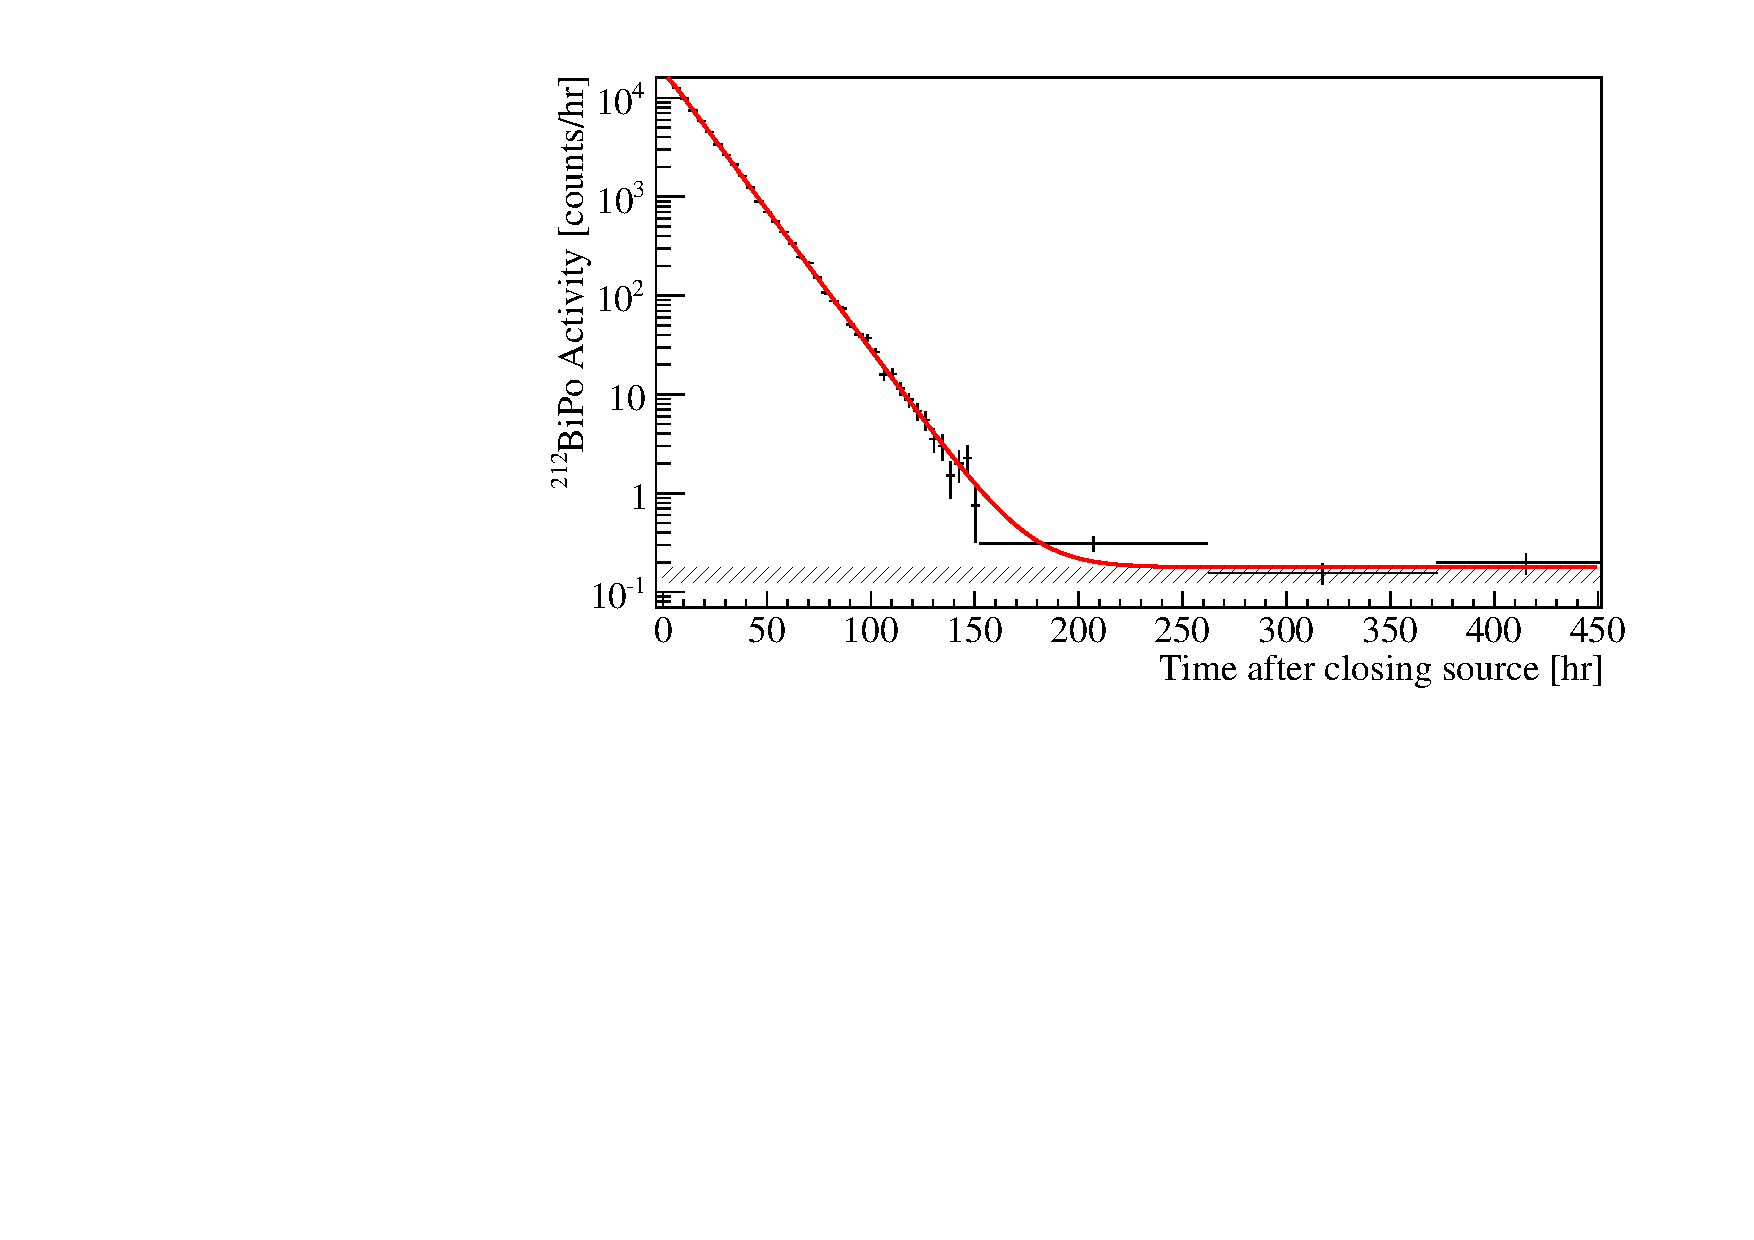
\includegraphics[trim = 10 5 40 15, clip = true,width = 0.8\columnwidth]{figures/chapter_five/bipo_background_sintered.pdf}
\caption{Decay to background of $^{212}$BiPo in the Si PIN diode for the measurement of the sintered filter. An exponential and a constant are fitted to the data. The band is the previously measured background of the detector.}
\label{fig:bipo_background}
\end{figure}

\begin{table}[htb]
\centering
\caption{Measurement results for the 0.5 micron sintered and ceramic filters}
\label{tab:filter_limits}
\renewcommand{\arraystretch}{1.2}
\begin{tabular}{lccc}
\hline\hline
Filter & Exposure & Fitted half-life & Fitted background \\ \hline
Sintered & $39\1{hr}$ & $(10.64\pm0.11)\1{hr}$ & $(49\pm8)\1{\mu Bq}$\\
Ceramic & $93\1{hr}$ & $(10.51\pm0.60)\1{hr}$ & $(46\pm8)\1{\mu Bq}$\\
\hline\hline
\end{tabular}
\end{table}

Both background values show some increase over the rate measured before this experiment, but in neither case is the increase statistically significant ($1\sigma$ for the sintered filter, $0.43\sigma$ for the ceramic filter). However, we can still (conservatively) attribute these small increases to some released \Ra, in which case we can limit the release of \Ra~to $<0.65\1{atoms/day/kBq}$ for the sintered filter and $<0.21\1{atoms/day/kBq}$ for the ceramic filter. Thus we see that both filters are highly effective at preventing the release of $^{224}$Ra from the source.

A more direct measurement of filter efficiency was performed by placing two identical 90~micron sintered filters in series in the gas system immediately after the source vessel. After recirculating xenon gas at 6.5~SLPM through the source and filters for 100~hours, the two filters were then placed on top of the Si PIN diode to measure any $\alpha$-activity coming off of them that could be attributed to \Ra. A total of 4~days of data were taken. The spectra of the two filters is shown in Figure~\ref{fig:twofilters}. While the first filter showed an activity of $(55.4\pm2.1)\1{mBq}$ of \Ra, the second filter that was placed immediately downstream of the first only showed an activity of $(1.63\pm0.18)\1{mBq}$ of \Ra. Both numbers are corrected for the activity at the time of source closing. Hence, their ratio directly gives the filter efficiency. This value is independent of systematic uncertainties such as the collection efficiency of the Si PIN diode, geometrical effects, etc. We thus find these 90~micron sintered filters to retain $(97.1\pm0.3)$\% of \Ra~flushing through them.

\begin{figure}[htb]
\centering
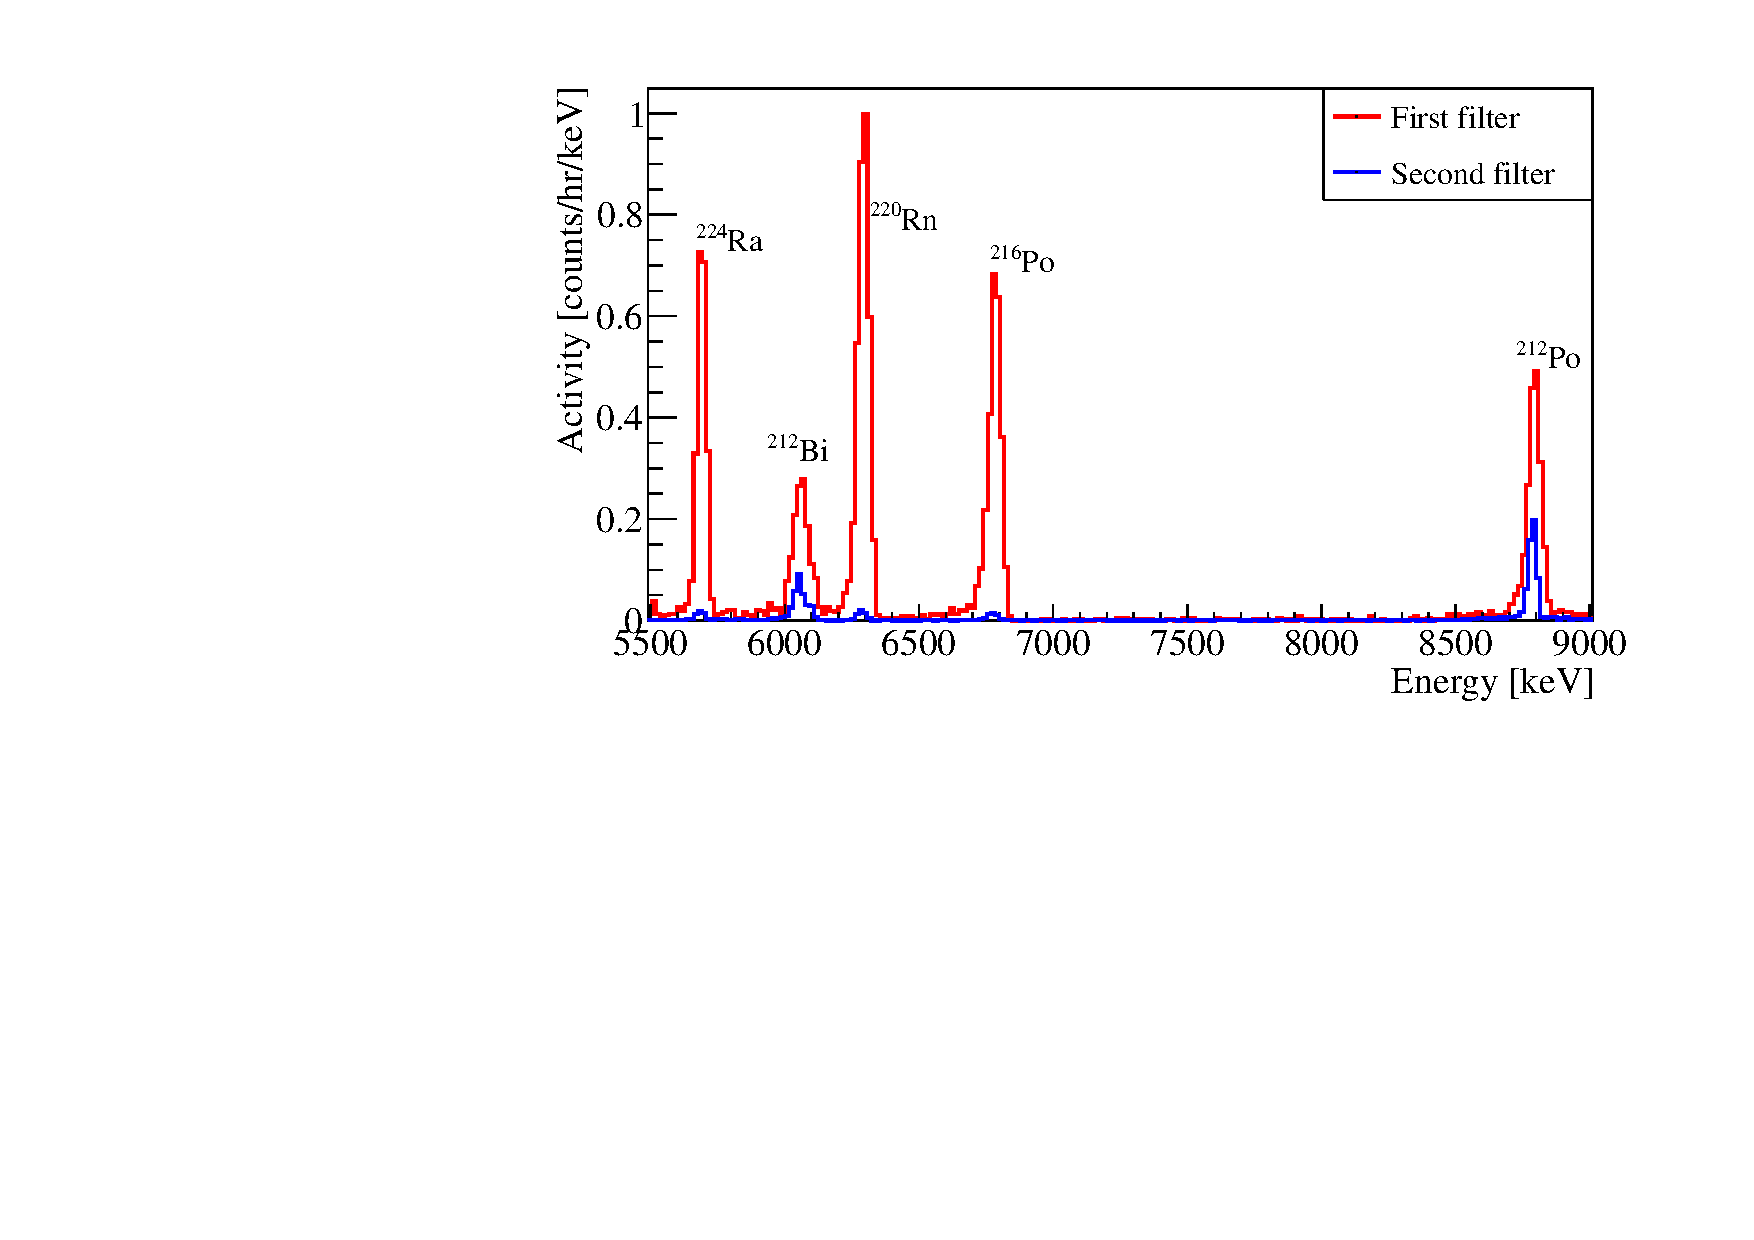
\includegraphics[trim = 5 0 40 20, clip = true,width = 0.8\columnwidth]{figures/chapter_five/twofilters.pdf}
\caption{Energy spectrum taken with the Si PIN diode from two sintered filters that were placed in series directly after the source in a xenon gas recirculation system.}
\label{fig:twofilters}
\end{figure}

\section{Mixing in a Liquid Xenon Detector}

A liquid/gas xenon TPC was used to test the injection of \Rn~into a liquid xenon detector. The detector was designed with a long drift length of 17~cm and a diameter of 80~mm. Each end of the drift chamber is monitored by 7~Hamamatsu R8720 photomultiplier tubes (PMTs). The walls of the TPC are constructed of a single cylinder of PTFE, for use as a UV~light reflector, with field shaping electrodes embedded inside the PTFE walls. The drift and charge amplification fields are applied with transparent meshes at the ends of the TPC to allow for high optical collection. For the measurements presented here, the detector was operated in a single-phase mode, with the full detector flooded with liquid xenon. This setup is sufficient to demonstrate that \Rn~can be flushed into the detector before decaying so that the subsequent \Pb~beta decays can be used as an internal calibrator. The detector was filled with about 3~kg of liquid xenon, which was continuously recirculated through a high-temperature zirconium getter to remove electronegative impurities. The recirculation is done in the gas phase using 1/2" VCR piping with a heat exchanger in the xenon loop~\cite{Giboni:2011wx}, constituting a setup very similar to that of the XENON1T experiment~\cite{Aprile:2012jh}. The \Rn~source vessel was connected to the gas recirculation system such that the gas could be flushed past the source or bypass it. Figure~\ref{fig:recirc} shows a schematic of the detector, purification loop, and \Rn~source. About 5~m of piping connected the \Rn~source to the TPC.

\begin{figure}[htb]
\centering
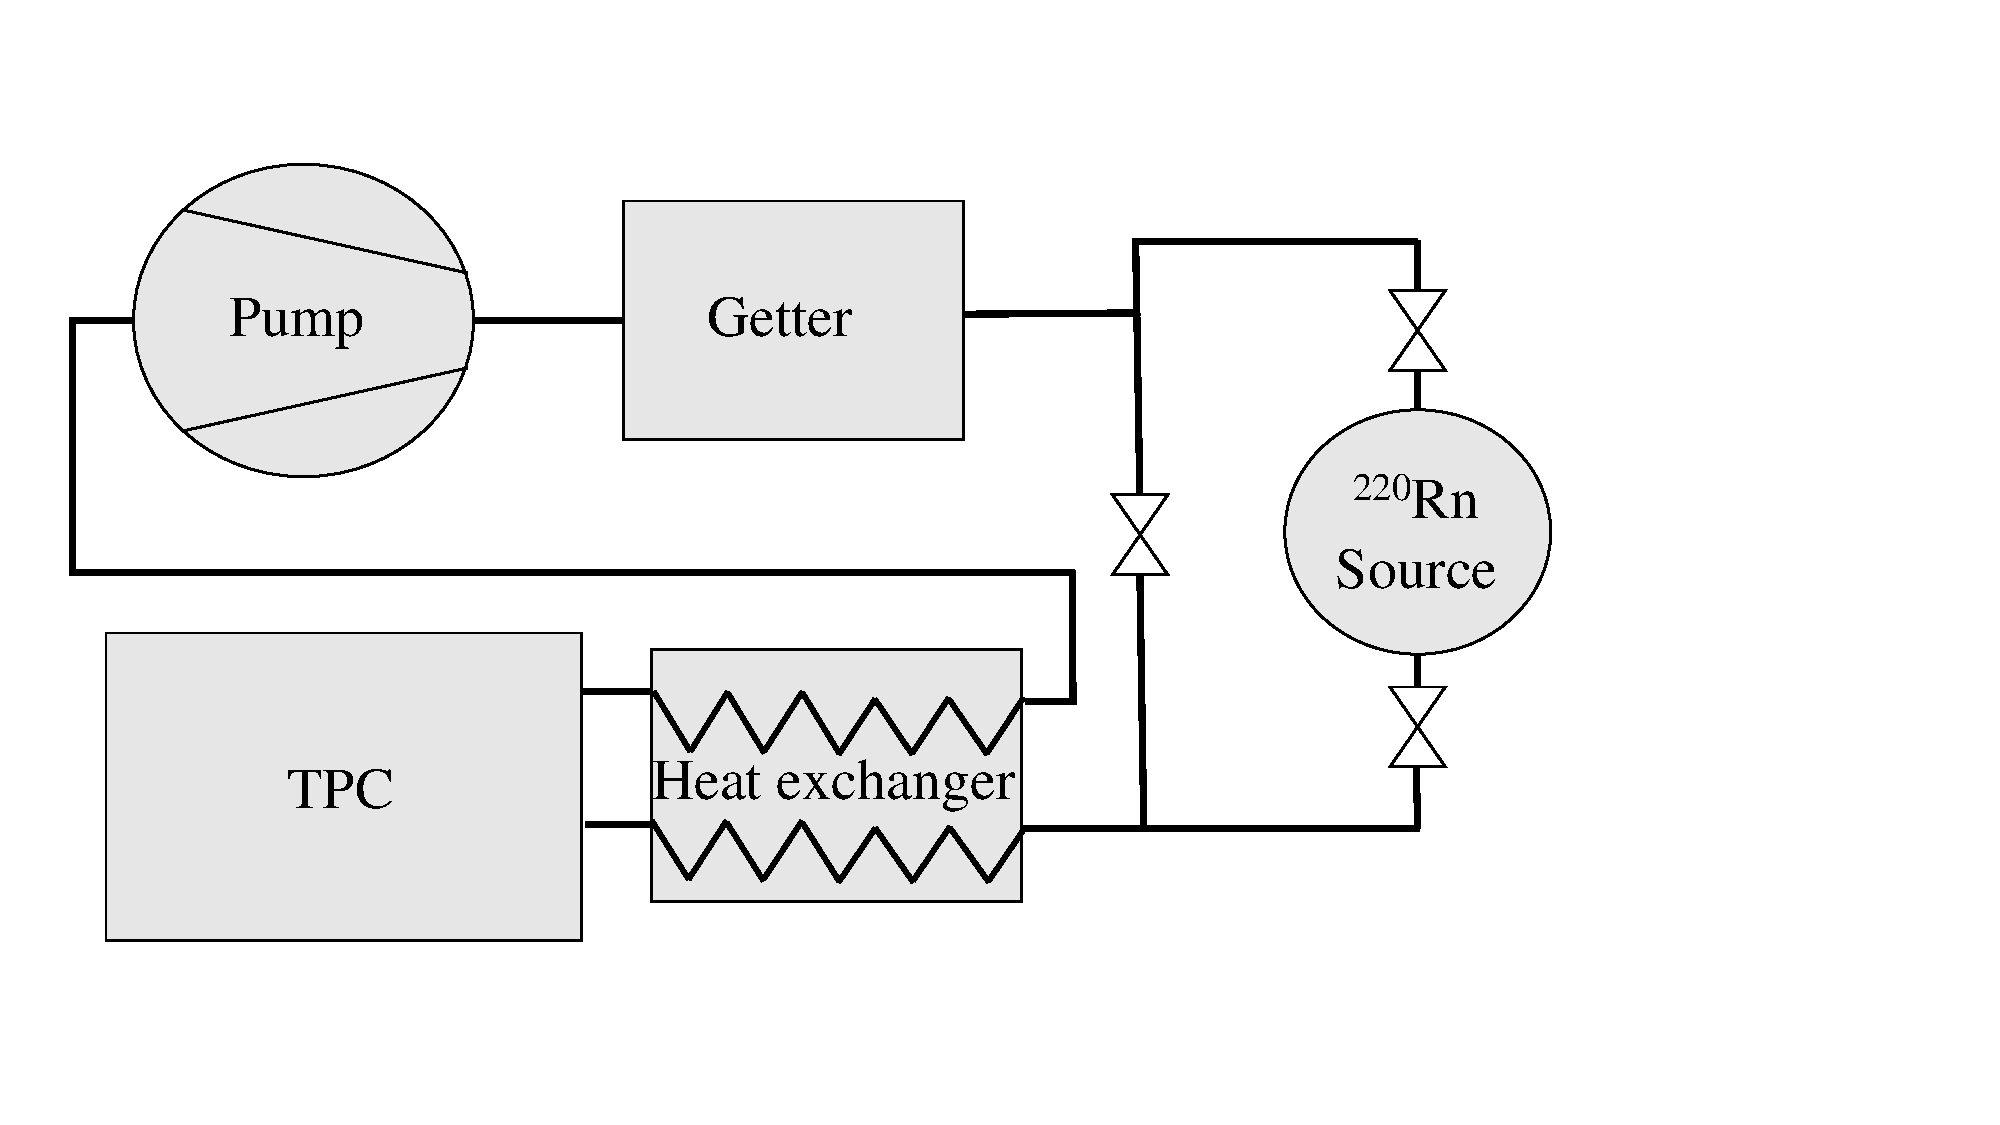
\includegraphics[trim = 30 55 210 75, clip = true,width = 0.8\columnwidth]{figures/chapter_five/recirc_schematic.pdf}
\caption{Schematic of the recirculation loop for the liquid xenon detector measurement. The liquid is evaporated in the heat exchanger and is pumped through the purifier, where it can then be flushed past the \Rn~source or injected directly back to the detector.}
\label{fig:recirc}
\end{figure}

To prove that the \Rn~could be mixed into the detector, the source was opened for 22.8 hours, injecting the doped gas. By monitoring the trigger rate of the detector in single phase operation, it was possible to observe the arrival of the dopants into the liquid xenon target. Data were acquired for 2.9~days surrounding this opening to determine the background before opening, and to monitor the decay of the injected \Pb~after the source was closed. The resulting trigger rate evolution is shown in Figure \ref{fig:Rates}. The background trigger rate of 200~Hz quickly rose to a saturated rate of around 550~Hz after the source was opened, showing that the activity of the source was entering the liquid xenon target. After the source was closed, the trigger rate quickly dropped to 450~Hz, after which it decayed toward the background rate.

\begin{figure}[htb]
\centering
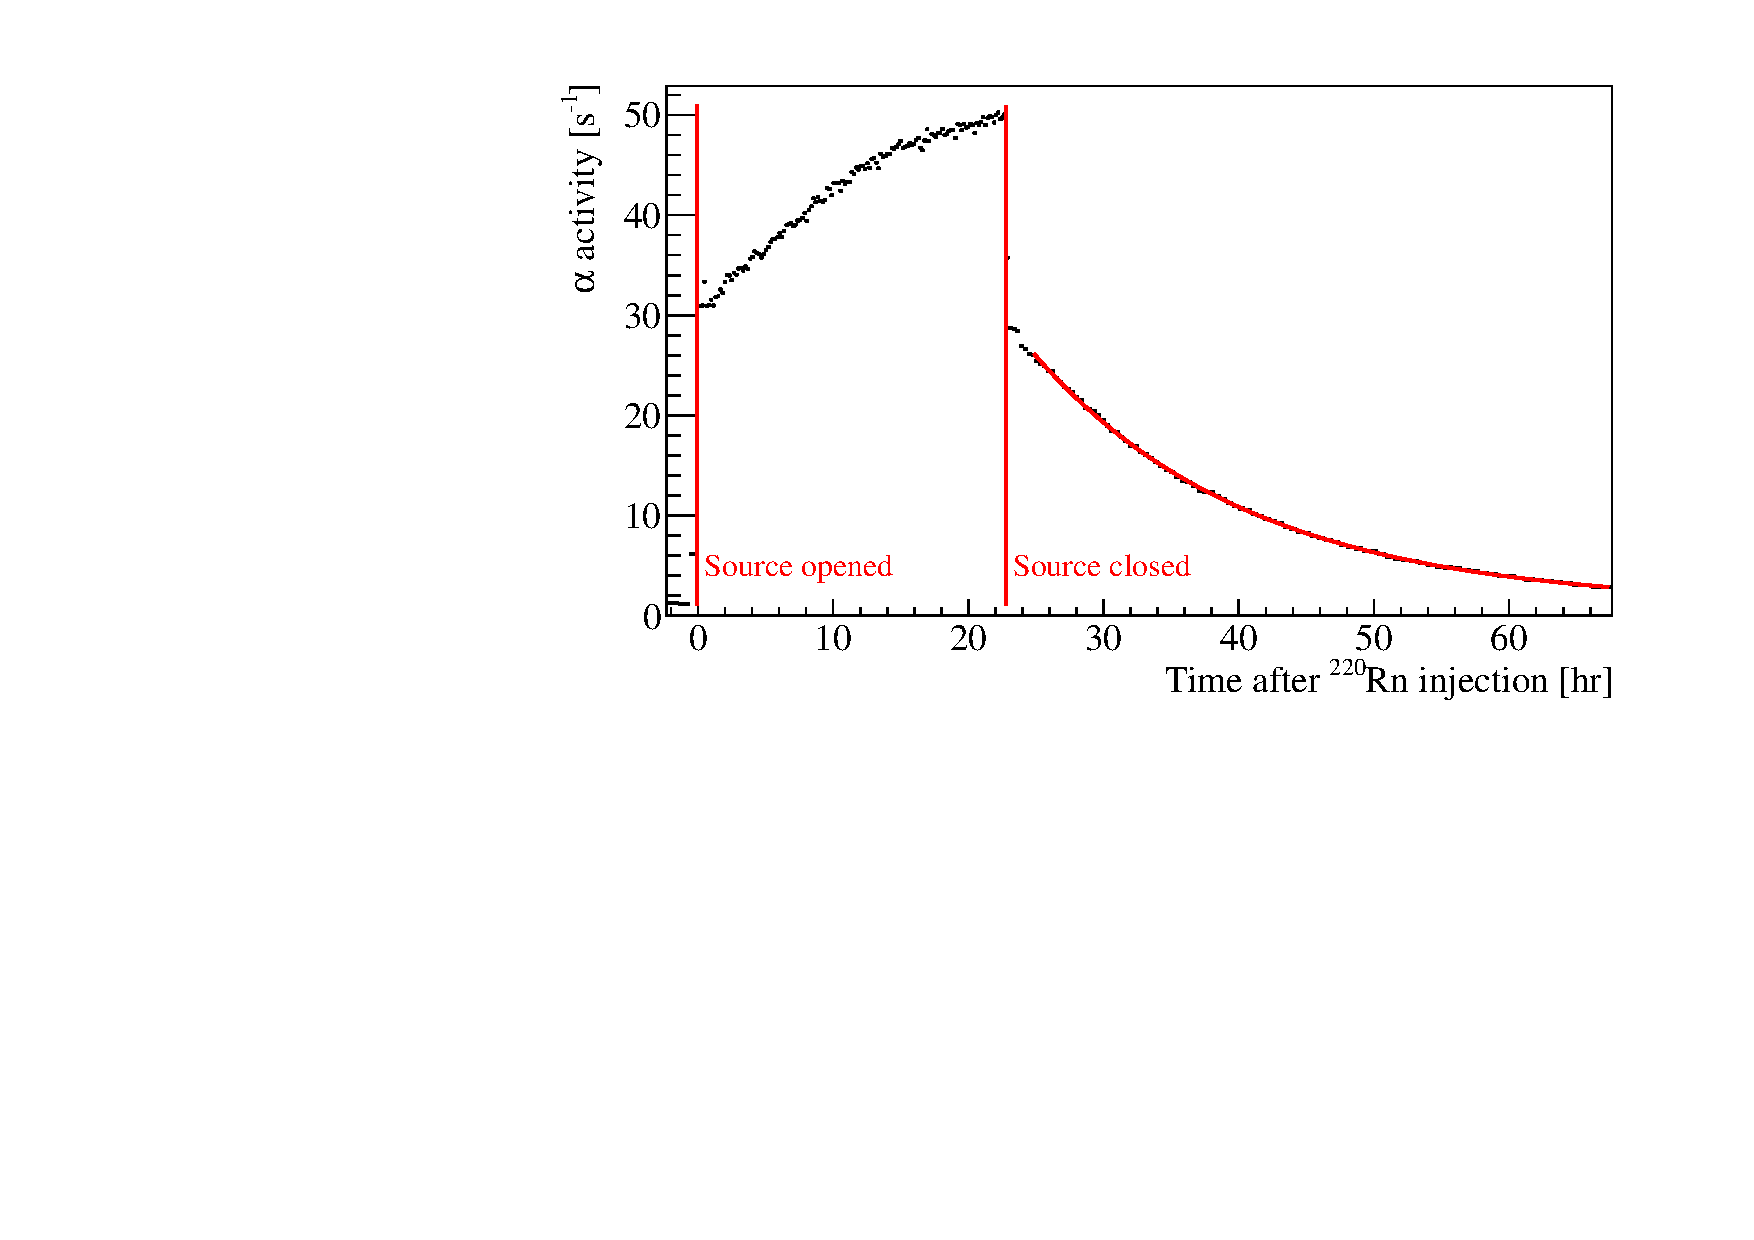
\includegraphics[trim = 5 5 55 15, clip = true,width = 0.8\columnwidth]{figures/chapter_five/tpc_rate.pdf}
\caption{Trigger rate in the liquid xenon detector before, during, and after source exposure. The spike in the rate after opening the source clearly shows the introduction of activity into the target volume, and the decay after it the source was closed indicates the presence of \Pb.}
\label{fig:Rates}
\end{figure}

The data acquisition system was not optimized for measuring high rates in a single phase operation, resulting in a large rate-dependent dead time. This impedes our determination of the actual activity in the target volume, as well as our ability to fit the observed decay to a single exponential. However, this measurement is clearly sufficient to demonstrate three major features of this source: first, \Rn~emanates from the source and can be mixed into a liquid xenon detector. Second, a low activity source is capable of introducing enough activity to be measured even above a high background rate. Third, the decay after the source is closed demonstrates the presence of \Pb~in the liquid target, a requirement to use this source for calibration of the low-energy region in a dark matter search.

\section{Interpretation}

\begin{table}[htb]
\centering
	\caption{Summary of all measurements of emanation rates, given in units of atoms/min/kBq.}
	\label{tab:summary}
	\begin{tabular}{lcc}
		\hline \hline
		Measurement & \Th & \Ra \\ \hline
		$\gamma$ measurements of filters, Section~\ref{sec:tuv}  & $<34$ & $<0.66$ \\
		& $<0.4$ & $1.9\pm0.6$ \\
		Pipe contamination, Section~\ref{sec:flush} & $<47$ & $1.53\pm0.04$ \\
		Radon monitor, Section~\ref{sec:diode} & $<0.008$ & $3.9\pm1.3$ \\
		Si PIN diode, Section~\ref{sec:diode} & $270\pm12$ & $16926\pm6$ \\
		Sintered filter, Section~\ref{sec:filter} & N/A & $<4.5\times10^{-4}$ \\
		Ceramic filter, Section~\ref{sec:filter} & N/A & $<1.5\times10^{-4}$ \\
		\hline \hline
	\end{tabular}
\end{table}

Table~\ref{tab:summary} summarizes the various measurements. The two $\gamma$ measurements of filter deposition and the measurement of pipe contamination are methodologically very similar, yet the results are strikingly different. Additionally, the measurement using the Si PIN diode are orders of magnitude different. The apparent inconsistency between the $\gamma$ measurements and pipe contamination can be attributed to deposition of \Ra~in the 1/2" piping: in the first two measurements, 18~cm and 8~cm of piping were present respectively in between the source vessel and filter, while the copper pipe was less than 1~cm from the source (leaving just enough space to cold-weld the copper). In the second $\gamma$ measurement, the flow through the source vessel and the filter was laminar, whereas the flow was turbulent for the pipe contamination measurement. Due to its extremely high reactivity, radium will bond readily to pipe walls. This is facilitated by turbulent flow, while in laminar flow, the slow process of radial diffusion will impede the plate-out of \Ra. As the second $\gamma$ measurement and the pipe contamination measurement are consistent, we attribute the discrepancy of the first $\gamma$ measurement to the different conditions of the gas flow.

For the measurements of filter efficiency, the limits presented for the ceramic and 0.5~micron sintered filters are very satisfactory, while in the two-filter measurement, the 90~micron sintered filters are only 97\% efficient. However, at the time of this measurement, the source had an activity of around 60~kBq. Hence, the activity seen in the first filter ($55.4\pm2.1\1{mBq}$) shows a drastic reduction in the activity after only a few centimeters of piping. From this, we can conclude that even though the source gives off very large amounts of \Ra~and \Th~(as shown by the Si PIN diode measurement), only a vanishing percentage makes it out of the source vessel. With these sources being used in a fluid stream, one may thus expect the vast majority of \Ra~and \Th~to plate out in any connecting piping.

\section{Conclusions}

We have presented a versatile \Rn~source for the internal calibration of low-background detectors and demonstrated its suitability. Stray emanation was found to be $<0.008\1{atoms/min/kBq}$ for \Th~and $(1.53\pm0.04)\1{atoms/min/kBq}$ for \Ra, which can be reduced to $<10^{-3}\1{atoms/min/kBq}$ through the use of an additional filter. We have demonstrated that the \Rn~activity can be mixed under realistic conditions in a liquid noble gas detector. The source provides the means by which to calibrate the electronic recoil band in liquid noble element dark matter detectors at low energies, characterize the important radon backgrounds, map fluid dynamics in the liquid target and possibly calibrate the Q-value of $^{136}$Xe double-beta decay.



%\chapter{The radon veto}~\label{ch:rnveto}

If it is possible to follow atoms of \Po~around the detector, the next step is to follow atoms further down the decay chain. If \Pb~atoms can be followed and their decays identified, these events can be removed from the analysis. As \Pb~is the dominant background source in the dark matter region of interest, this has the possibility to significantly boost the sensitivity of the experiment at a marginal cost in exposure. We exploit the fact that \Pb~is part of a larger decay chain, lending physical significance to the times and positions of its decays.

We will begin with a brief review of the relevant portion of the decay chain of primordial uranium, as shown in Figure~\ref{fig:useries}. \Pb~decays to the ground state of $^{214}$Bi with a branching ratio of $11.0\%$, and a fraction of these decays lie in the dark matter signal region of interest. This is the primary cause of background in this energy range.

\begin{figure}[htb]
    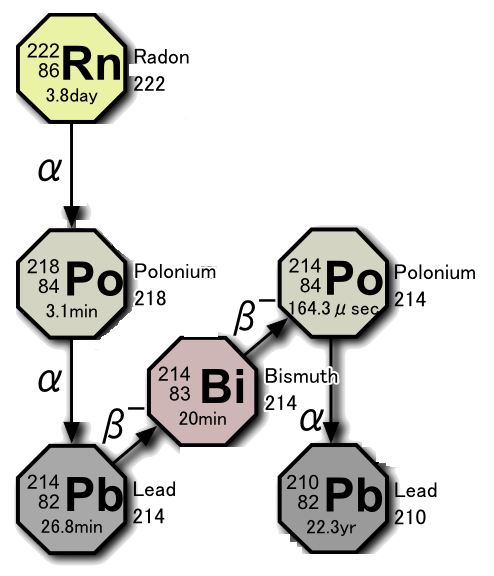
\includegraphics[width=\textwidth]{figures/rnveto/uranium_series}
    \caption{A section of the decay chain of primordial ${}^{238}$U. Atoms of \Rn~emanate out of impurities in the metals used in detector construction and mix throughout the xenon volume. Low-energy decays of \Pb~that decay directly to the ground state of $^{214}$Bi are the leading cause of background in the dark matter ROI.}\label{fig:useries}
\end{figure}

\section{Technique overview}

While there is nothing about a \Pb~event that is easily identifiable, its parent isotopes (\Rn, \Po) and daughtber (\BiPo) can be identified in analysis with relative ease using alpha spectroscopy or the BiPo timing structure. This allows us to bookend the \Pb~event with events that are more easily identified. With this information, an algorithm resembling one for track reconstruction mightb be employed to improve the confidence with which \Pb~events are tagged by identifying the decays of the parents and daughtber and looking for the convection streamlines that connect them. The \Pb~decay must happen somewhere on that streamline between the \Pb~and \BiPo. A simple representation of this is shown in Figure~\ref{fig:rnveto_schematic} where displacement due to convection is normalized out.

\begin{figure}[htb]
    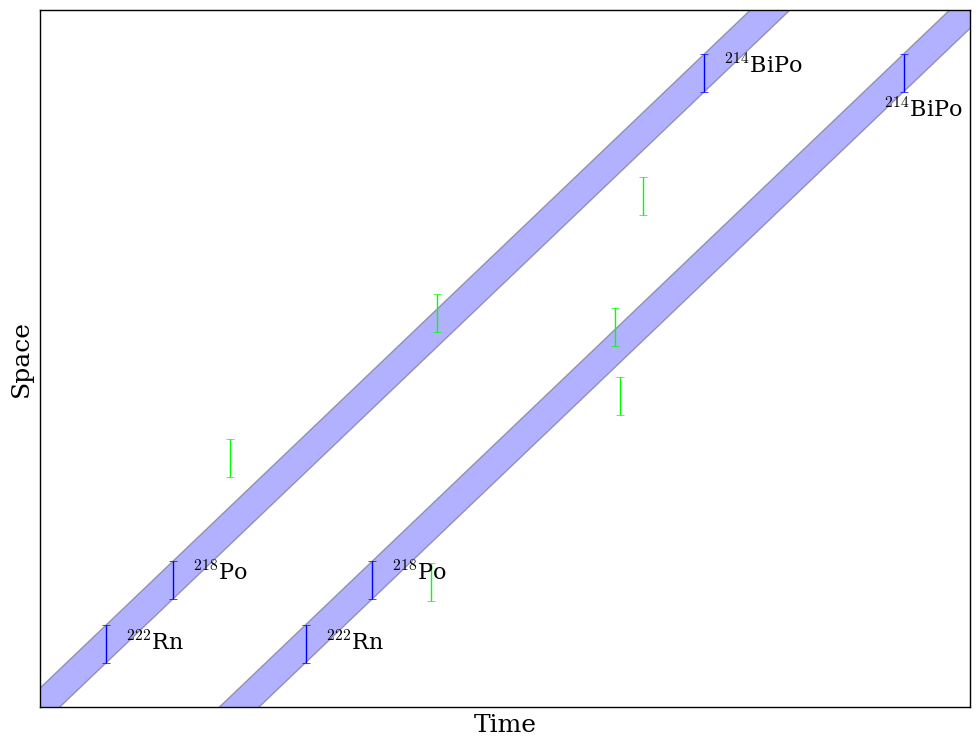
\includegraphics[width=\textwidth]{figures/rnveto/schematic}
    \caption{A simple schematic of how the radon veto works. Low-energy events (in green) due to \Pb~can be identified because they occur on streamlines (shaded regions) connecting \Rn, \Po, and \BiPo~events (in blue), while low-energy events due to other background sources occur at random.}\label{fig:rnveto_schematic}
\end{figure}

\section{Convection-agnostic approach}

To demonstrate a proof of this concept, we employ a convection-agnostic approach. In this method, a sphere is placed around every \Po~or \BiPo~event. Regardless of the size of the sphere or how long one watches it, some fraction of \Pb~decays will occur within it. The size of the sphere can be connected to the length of observation time by the average speed of convection, and the observation time can be chosen by a simple optimization to maximize the potential background reduction while minimizing the overall exposure cost.

The principle background to this Big Sphere method is that of false positives from random coincidence. This can be very easily quantified by placing spheres at random locations and random times within the detector, monitoring the sphere for the specified duration, and counting the number of times a low-energy event is observed. This can then be repeated using locations and timestamps of \Po~or \BiPo~events rather than at random. This allows for the clear quantization of the significant of the result. This was appllied to science run 0, with results shown in Figure~\ref{fig:bs_sr0}.

\begin{figure}[htb]
    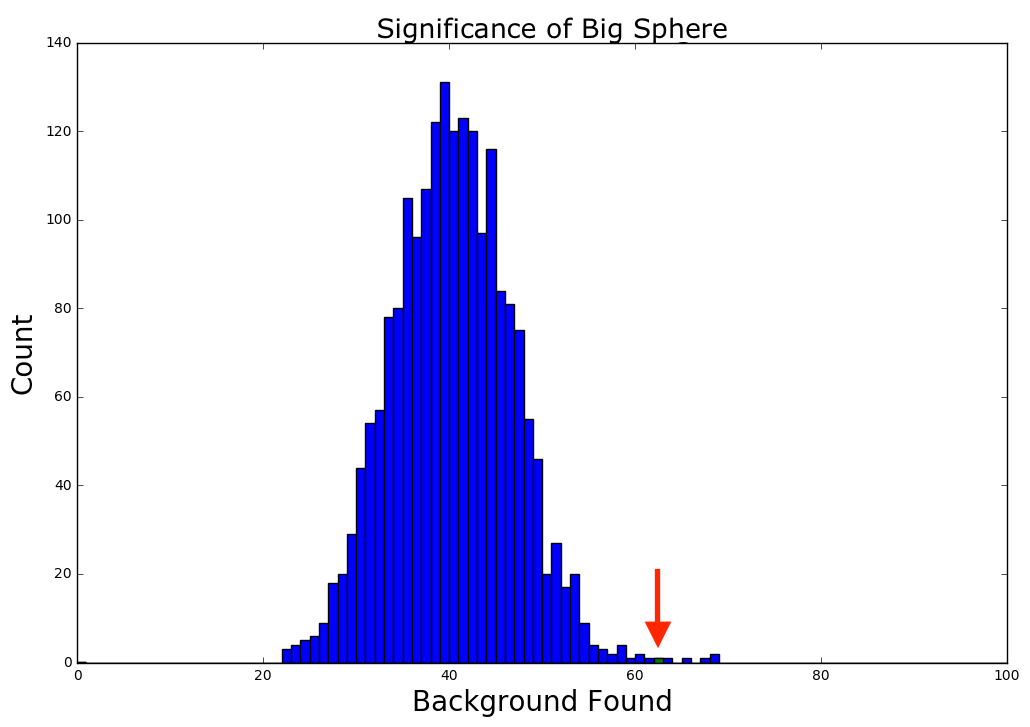
\includegraphics[width=\textwidth]{figures/rnveto/BigSphere}
    \caption{The background estimation for the convection-agnostic Big Sphere method for science run 0. The background from false positives is well-modeled with a binomial distribution. The number of events found by searching near \Po~and \BiPo~is XX. This has a p-value of YY, indicating a significant result.}\label{fig:bs_sr0}
\end{figure}

\section{Cloud approach}

The Big Sphere method has a number of limitations. Looking in all directions rather than just along the convection streamlines wastes a large amount of exposure, and in cases where multiple low-energy events are observed within the sphere it is impossible to know which is due to the \Pb. At most one can be due to \Pb, yet without additional information it is impossible to determine which. This additional information is from convection. If an event is on known fluid streamlines originating from the \Po~decay vertex or converging to the \BiPo~vertex, it is more likely to be \Pb~than if it occurred far from those streamlines or on otherwise impossible paths.

The computational cost of following these streamlines is non-trivial. It involves a numerical integration of a vector field, and doing this multiple times. Each \Rn~atom can potentially produce a low-energy \Pb~event, so streamlines around every \Rn~must be followed. At a decay rate of $\approx 2\,500\1{day^{-1}}$, a tonne-year of exposure will contain nearly $500\,000$ total \Rn~events. Streamlines from each of these events must be integrated for (on average) one hour, at sufficiently small timesteps to minimize integration errors.

\section{Diffusion-limited case}

The dominant uncertainties to the radon veto stem from the lack of complete knowledge of the convection pattern. However, we can explore the possibilities of the technique should a perfect understanding of convection be obtained. In this limit, the dominant uncertainties are from position reconstruction and diffusion.

\subsection{Diffusion effects}

When an event happens, we reconstruct its interaction vertex with a uncertainty of $5\1{mm}$ in r and $1\1{mm}$ in z. For reasons we will discuss shortly, we will take 2 sigma and double these. Thus, we assume this event happens somewhere in a cylinder of volume $\approx 630\1{mm^3}$. This cell will follow the convection lines through the volume, growing in time due to diffusion. We'll need a few values here:
\begin{itemize}
    \item $r_0 = 10\1{mm}$
    \item $h_0 = 2\1{mm}$
    \item Cell volume: $V(t=0) = \pi r_0^2h_0 = 630\1{mm^3}$
    \item Diffusion constant: $D = \frac{k_BT}{6\pi\eta r} = 1.7\times10^{-3}\1{mm^2/s}$
\end{itemize}

We find the diffusion constant via the Stokes-Einstein relation for diffusion of a spherical particle through a fluid at low Reynolds number~\cite{Sutherland:1905,Einstein:1905,Smoluchowski:1906}. $\eta$ is the viscosity ($0.5\1{mPa s}$~\cite{Legros:1965}) and $r$ is the radius of the particle in question (taken as $0.15\1{nm}$). The displacement of the atom from its initial location will be roughly given by $\Delta s = \sqrt{\pi Dt}$, and the increase in volume can be found by adding $\sqrt{\pi Dt}$ to both r and z. Thus

\begin{equation}
V(t) = \pi(r_0 + \sqrt{\pi Dt})^2(h_0 + \sqrt{\pi Dt})
\end{equation}

Starting from a decay of \Po, in one half-life of its daughtber ($\sim$30 min) the cell volume will increase by $2.1\1{cm^3}$ to $2.75\1{cm^3}$. If we see an ER event in this volume in the energy range we would expect from a \Pb~decay, we can cut this event (and stop following that cell as it is no longer a potential background event).

\subsection{Total vetoed volume}

The next value to calculate is what fraction of the active region we can follow. For that we need to calculate how many atoms we need to follow at any one time. As calculated above, we find that on average the detector will contain these populations:
\begin{itemize}
    \item $N_{Rn} = 13\,300$
    \item $N_{Po} = 7.5$
    \item $N_{Pb} = 66$
    \item $N_{Bi} = 48$
\end{itemize}

Atoms further down the decay chain will have slightbly reduced populations due to plateout and cathode cleaning, but these values are upper limits. The probability that we must still follow the atom in that volume $P(t) = \exp -\lambda t$ (if the atom decays, we no longer need to follow it), and the expression for the cell volume is given above.

If we wish to reduce the contribution of \Pb~to the low-energy background to the point where it becomes equivalent or subdominant to the other sources of ER background, this requires that we veto about 90\% of all low-energy lead events. This means we have to follow a cell for 3 or 4 half-lives, and for this reason we took 2 sigma of the position uncertainty (giving us 95\% of the atoms). The results change very little if we follow the atom around for an infinite number of half-lives. So, for the math we are about to do, we will integrate over all time, not just the few half-lives we need, and use the resulting closed-form expressions.

To find the average cell volume we integrate the volume $V(t)$ with the probability density $P(t) = \lambda \exp -\lambda t$ to get

\begin{equation}
\left< V \rightb> = \int_0^{\infty} \dd t\,V(t) P(t) = \int_0^{\infty} \dd t\,\pi(r_0 + \sqrt{\pi Dt})^2(h_0 + \sqrt{\pi Dt})\lambda\exp -\lambda t
\end{equation}

The result is

\begin{equation}
\left< V \rightb> = V_0 + a\sqrt{\chi} + b\chi + c\chi^{3/2}
\end{equation}

where:
\begin{itemize}
    \item $\chi = \frac{D}{\lambda}$ (units of $\n{mm^2}$)
    \item $a = \frac{\pi^{2}}{2} (r_o^2+2 r_0 h_0) = 690\1{mm^2}$
    \item $b = \pi^2 (2r_0 + h_0) = 220\1{mm}$
    \item$c = \frac{3}{4} \pi^{3}$
\end{itemize}

For \Pb, $\chi = 4\1{mm^2}$, so $\Delta V = 2.5\1{cm^3}$ or the total volume we must follow per atom is $V_0 + \Delta V = 3.1\1{cm^3}$. Given the average number of \Pb~atoms we expect to have, this will be a total vetoed volume of $140\1{cm^3}$. This is only $10^{-4}$ of the total active volume. We can also calculate the total volumes to track for the parent and daughtber isotopes, but this is only for tagging purposes as we have no need to veto events that aren't \Pb.

If we take a pessimistic approach where we follow each cell for four half-lives (regardless of whether or not the atom in it decays), we find a total vetoed volume of $V(4T_{1/2}) = 300\1{cm^3}$. Thus, the $140\1{cm^3}$ value is reasonable from this point as well.

\subsection{Pb-210}

As the half-life of $^{210}$Pb is long (22 years), in one half-life it can diffuse to anywhere in the TPC, so we cannot follow it.

\subsection{Effect of the drift field}

We expect the drift field to cause the motion of any charged daughtber products to diverge from that of the xenon bulk. This effect can be simulated, but measuring the charge on the daughtber ion will be difficult, and this uncertainty reduces the effectiveness of any simulation involving this aspect. In effect it will cause a net downward motion, which will move the ion into other streamlines (or potentially plate onto the cathode). Additionally, as we inject the liquid below the cathode, ions in the liquid will probably have difficulty passing through the cathode mesh and into the drift region.

EXO-200 found~\cite{Albert:2015vma} radon daughtber ion drift speeds of $\sim 1\1{mm/s}$ with a drift field of $350\1{V/cm}$, with ion neutralization time proportional to the electron lifetime. Additionally, they measured the fraction of radon chain decays that leave the daughtber in an ionized state. In XENON100 the ion drift was a small correction to the $\sim 8\1{mm/s}$ flow speed.

In the two extreme cases (zero and infinite electron livetime), the ions will neutralize immediately and then follow the known fluid streamlines, or never neutralize, drift down, and plate onto the cathode, where they won't contribute to the background in the fiducial volume. In the more likely intermediate case, ions will drift downwards until they neutralize and then follow the fluid.


%
\chapter{Recommendations}

Buy low. Sell high.


\appendices

\bibliographystyle{plain}
\bibliography{bibliography}

%  A vita is required only in a doctoral dissertation.
%

\begin{vita}
    [Put a brief autobiographical sketch here.]
\end{vita}


\end{document}
